\documentclass[12pt]{article}

\usepackage{sbc-template}

\usepackage{graphicx,url}

\usepackage[english]{babel}   
%\usepackage[latin1]{inputenc}  
\usepackage[utf8]{inputenc}  
% UTF-8 encoding is recommended by ShareLaTex
\usepackage{verbatim}
\usepackage{listings}
\usepackage{xcolor}
\usepackage{graphicx}
\usepackage{listings}
\usepackage[]{algorithm2e}
\usepackage{color}
\usepackage{amsmath}
\usepackage{amsfonts}
\usepackage{multirow}
\RestyleAlgo{ruled}
\usepackage{fancybox}
\usepackage{siunitx}
\usepackage{subcaption}
\usepackage{fixltx2e}
\usepackage{standalone}
\usepackage{float}

\graphicspath{ {Figures/} }

\newcommand\norm[1]{\left\lVert#1\right\rVert}
\definecolor{verde}{rgb}{0,0.5,0}
\DeclareMathAlphabet{\mathpzc}{OT1}{pzc}{m}{it}
%para customizar o código (ver https://en.wikibooks.org/wiki/LaTeX/Source_Code_Listings)
\lstset{language=C, %defina a linguagem usada no trabalho
              belowcaptionskip=1\baselineskip,
                breaklines=true,
                frame=false,
                xleftmargin=\parindent,
                showstringspaces=false,
                basicstyle=\footnotesize\ttfamily,
                keywordstyle=\bfseries\color{green!40!black},
                commentstyle=\itshape\color{purple!40!black},
                identifierstyle=\color{blue},
                stringstyle=\color{orange},
                numbers=left,
            }

\sloppy

\title{Virtual Reality 1}

\author{Dongho Kang, Jaeyoung Lim, Soomin Lee and Jaeryeong Choi}

\address{\{kangd, jalim\}@ethz.ch}

\begin{document} 

\maketitle
\documentclass{standalone}
% Load any packages needed for this document
\begin{document}

\section{Chapter 1: Introduction into Virtual Reality}

\setcounter{subsection}{1}	% 1.1 omitted

%----------------------------------------------------------------------------------------
\subsection{The development of the computer}

\begin{itemize}
	\item \textbf{the constant increase of computational power available in modern computer} $\rightarrow$ today's abundance of virtual reality. 
\end{itemize}

\subsubsection*{Numbers}
\begin{itemize}
	\item 6000 years ago: the earliest use of numbers. 
		\begin{itemize}
			\item 3300 B.C. Egypt: battle report in hieroglyphs.
		\end{itemize} 
	\item number system 
		\begin{itemize}
			\item The first number systems exist in hieroglyphs \\ e.g. $1=\textit{line}$, $10=\textit{horseshoe}$ ...
			\item Roman: 

				\begin{table}[h]
				\centering
				\begin{tabular}{| c | c | }
				\hline
				I $= 1$		& V $= 5$ 	\\
				\hline 
				X $= 10$	& L $= 50$ 	\\
				\hline							
				C $= 100$	& D $= 500$ \\
				\hline					
				M $= 1000$ 	& 			\\		
				\hline					
				\end{tabular}
				\end{table}
				
				\begin{center}
				$2388 =$ MMCCCLXXXVIII
				\end{center}
			
			\item \textbf{Addition-system} (Roman, Greeks, Syrians, Slavic tribes ...): large numbers are made by adding up the symbols 
			\item \textbf{Indo-Arabian}: the system used until today (1, 2, 3, 4, 5, 6, 7, 8, 9, 0)
				\begin{itemize}
					\item more complicated calculation can be performed very easily.
					\item very forgery-proof
					\item 6th century: Indian to Mesopotamia (Severus Sebakt)
					\item 10th century: came to Europe (Leonardo Fibonacci)
					\item 16th century: printing numbers were introduced (Adam Ries and Albrecht Dürer) 
				\end{itemize}				
		\end{itemize}
\end{itemize}

\subsubsection*{Calculation}

\begin{itemize}
	\item First means to calculate
		\begin{itemize}
			\item calculating with the fingers - Rome: 40 finger positions, displays up to 200000 (Note: digitus(finger in Latin) $\rightarrow$ digit (eng.)
			\item tally stick (Europe), knots (native Americans)
		\end{itemize}
	\item The first scientific calculation: \textbf{abacus} 
	\item \textbf{Written calculation became popular (since 15c)}
		\begin{itemize}
			\item \textbf{easy and fast}: eased calculations and reduced the required time.
			\item \textbf{accurate}: lowered the failure rate.
			\item Adam Ries: make math accessible to everybody.
		\end{itemize} 
\end{itemize}

\subsubsection*{Calculation machine (17c ~)}

\begin{itemize}
	\item to make calculation more easy, fast and accurate
	\item the first calculation machine (W. Schickardt, 17c) \textbf{Figure 1.16, page 1-12}
		\begin{itemize}
			\item add numbers up to 6 digits
			\item multiplication were possible. 
			\item toothed gears and slide rules. 
		\end{itemize}
	\item B. Pascal(1623 - 1662) \textbf{Figure 1.17, page 1-12}
		\begin{itemize}
			\item made money with calculation machine (the first one) 
			\item add and subtract numbers with 8 digits. 
			\item more than 50 pieces were produced. 
		\end{itemize}
	\item G. W. Leibniz (1646 - 1716) \textbf{Figure 1.18, page 1-12}
		\begin{itemize}
			\item introduced the machine suitable for all four basic calculation. 
		\end{itemize} 
	\item The calculating machines of 18c: more reliable, but became a piece of jewelry than a device for daily use \textbf{Figure 1.19, page 1-13}
	\item C. X. Thomas (1785 - 1870) \textbf{Figure 1.20, page 1-13}
		\begin{itemize}
			\item precise, efficient and ergonomic.
			\item ``arithmometer": multiplied two numbers with 8 digits in 18 sec.
			\item more improved later 	
		\end{itemize}
	\item \textbf{Programmable calculation machines} (C. Babbage, 1792 - 1871)
		\begin{itemize}
			\item punched cards for programming. 
			\item could run the program autonomously.
			\item used steam machine and weights, but failed to realize his idea. 
			\item \textbf{separated counting mechanism, calculation mechanism and storage} (origin of 20c computer architecture)
		\end{itemize}
	\item \textbf{Calculation machine with electrical devices} (H. Hollerith, 1860 - 1929)
		\begin{itemize}
			\item \textbf{Figure 1.22, page 1-15}
			\item control mechanism activated by electrical devices (relays, motors ... ) with punched cards: hole $\rightarrow$ closed (1) / no hole $\rightarrow$ opened (0)
			\item American Census in 1890: shorten the time for analysis 7 yrs $\rightarrow$ 1 yrs
			\item founded IBM
		\end{itemize}
\end{itemize}

\subsubsection*{Computer era (20c ~)}

\begin{itemize}
	\item Theoretical background of the first programmable electrical calculation machine (The first computer): \textbf{L. Couffignal and A. M. Turing}
	\item The first computer: \textbf{ZUSE Z3} by K. Zuse (1941)
		\begin{itemize}
			\item Z1 (didn't work) $\rightarrow$ Z2 (simple tests) $\rightarrow$ Z3 
			\item could handle 64 numbers with 22 digits. 
			\item 2600 relays and 8 line punched tape ($\rightarrow$ tube/transistor was used later)
			\item Z4 (1950s) worked at ETH 
		\end{itemize}	
	\item \textbf{The first encryptor \& decryptor}: Enigma vs Colossus (1941)
		\begin{itemize}
			\item Colossus: the first electronic computer
			\item MARK 1 (1943) in US
			\item MARK 2 (1944) in US
		\end{itemize} 
	\item \textbf{ENIAC (1946)} \textbf{Figure 1.25, page 1-16}
		\begin{itemize}
			\item J. P. Eckert, J. Mauchley and H. H. Goldstine
			\item von Neumann architecture
			\item 18000 tubes, 1500 relays, 1000 capacitors and 6000 switch.
			\item very fast... 0.0002 sec for addition, 0.0028 sec for multiplication 
		\end{itemize}
	\item \textbf{Transistor} invented (1948) \textbf{Figure 1.26, page 1-17}
		\begin{itemize}
			\item \textbf{smaller, faster, less heat, longer life cycle, manufactured automatically}
			\item \textbf{switch: relays $\rightarrow$ tubes $\rightarrow$ transistor} (electronics)
			\item TRADIC (1955): the first computer used transistors
		\end{itemize}   
	\item \textbf{single chip computer(CPU)} (Integrated Circuits) 
		\begin{itemize}
			\item 4-bit processor INTEL and Texas Instrument in 1970
			\item 8-bit (1972), 16-bit (1978) ... now 32 bit / 64 bit
		\end{itemize}
	\item \textbf{Personal Computer (PC)}
		\begin{itemize}
			\item because of IC, the size of computers could be drastically reduced
			\item Kenbak1 (1971): the first single chip computer
			\item ALTAIR 880 (1974): mass market
				\begin{itemize}
					\item \textbf{Basic}: a new programming language developed for ALTAIR
				\end{itemize}
			\item (1980s) Apple II \& Commodore PET: the first commercial success
			\item Lisa and Macintosh : GUI
			\item IBM PC became very popular
		\end{itemize}
	\item SGI were used for high-performance computer graphics: Virtual Reality...
\end{itemize}

\subsubsection*{Moore's law and the development of computer}

\begin{itemize}
	\item \textbf{Moore's law} (1965): \textbf{the amount of transistors} in a computer is doubled all 18 months. \textbf{Figure 1.34, page 1-22}
	\item but also the required space for the transistors becomes smaller and smaller. i.e. \textbf{the available memory per chip} is increases: x4 every 3 yrs
	\item \textbf{chip size} also increases: x2 every 10 yrs 
	\item \textbf{CPU speed} increases: x2 every year
\end{itemize}

\begin{figure}[h]
	\centering
	\begin{subfigure}[b]{0.45\textwidth}
		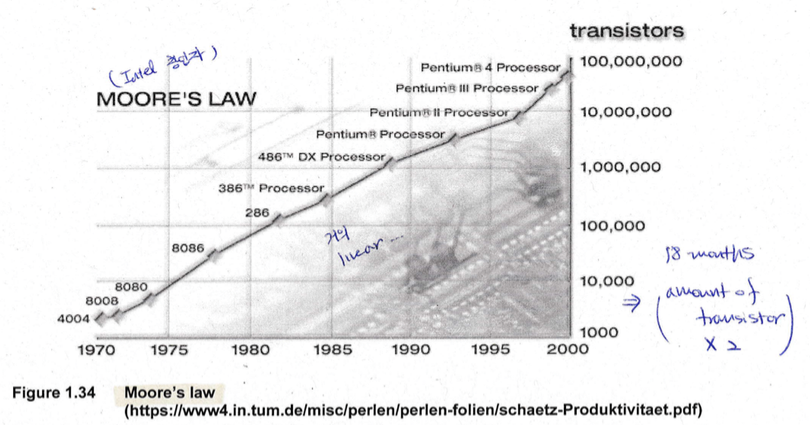
\includegraphics[width=\linewidth]{1_34}
	\end{subfigure}
	\begin{subfigure}[b]{0.45\textwidth}
		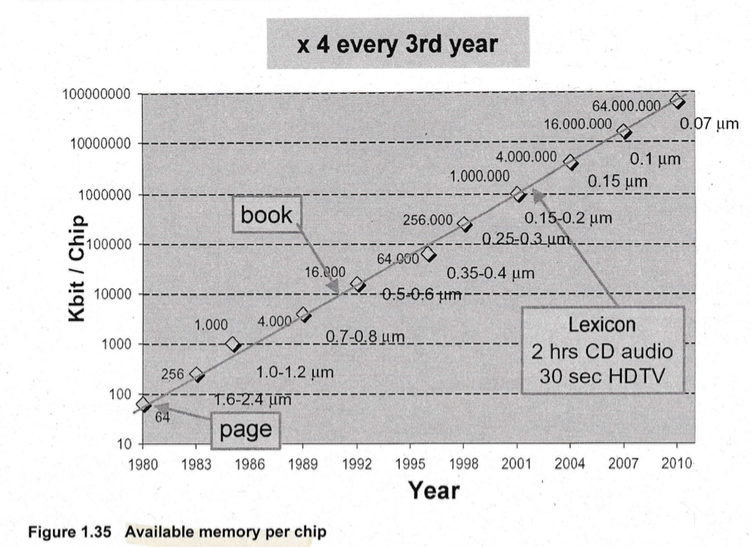
\includegraphics[width=\linewidth]{1_35}
	\end{subfigure}
	\begin{subfigure}[b]{0.45\textwidth}
		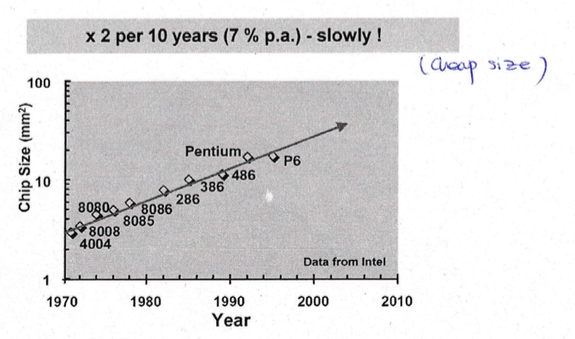
\includegraphics[width=\linewidth]{1_36}
	\end{subfigure}
	\begin{subfigure}[b]{0.45\textwidth}
		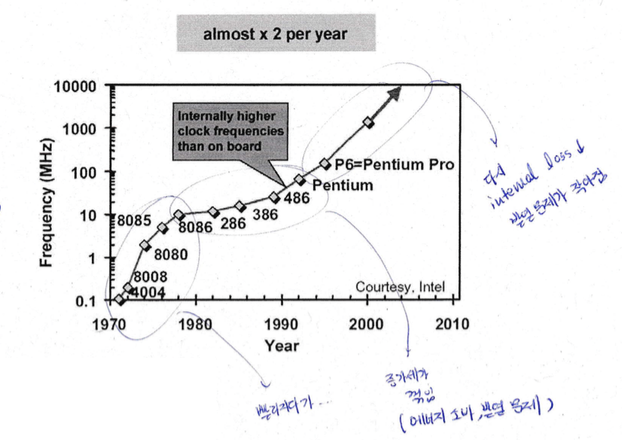
\includegraphics[width=\linewidth]{1_37}
	\end{subfigure}
\end{figure}

\subsection{Definitions}

\begin{itemize}
	\item Reality (exist): real object $\gg$ virtual object
	\item Mixed Reality 
		\begin{itemize}
			\item Extended Reality (Augmented Reality): real obj $>$ virtual obj
			\item Extended Virtuality (Augmented Virtuality): real obj $\leq$ virtual obj
		\end{itemize}
	\item Virtual Reality (non exist): real obj $<$ virtual obj
	\item \textbf{Note: Figure 1.39, page 1-25}
\end{itemize}

\begin{figure}[h]
	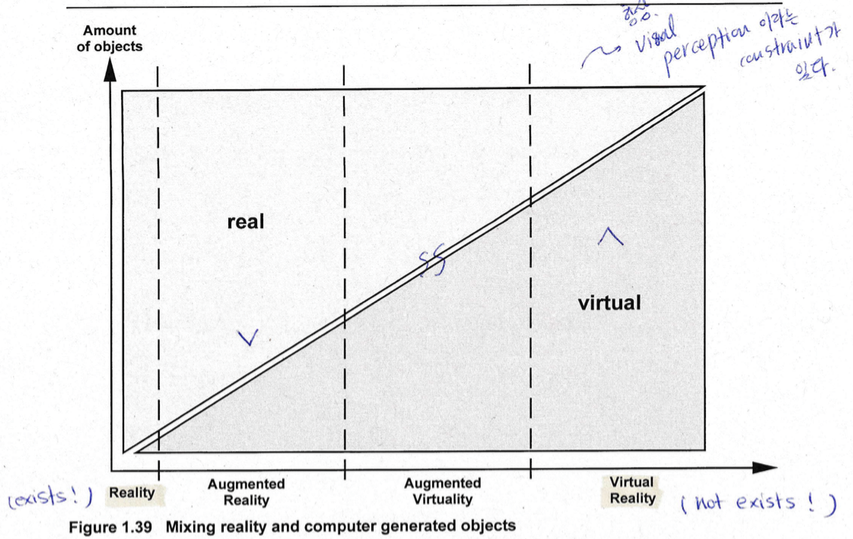
\includegraphics[width=\linewidth]{1_39}
\end{figure}

\subsubsection{Extended Reality (augmented reality)}

\begin{itemize}
	\item \textbf{real object $>$ virtual object}
	\item the computer generated objects are characterized by the fact but usually differ from reality in scale, shape or color.
	\item e.g. AR on copy machine: indicate parts to be fixed  
\end{itemize}

\subsubsection{Extended Virtuality (autmented virtuality)}

\begin{itemize}
	\item \textbf{real object $<$ virtual object}
	\item comparing to AR, virtual objects are much more detailed and fit much better to reality.
	\item e.g. Reconstruction of ruins \textbf{Figure 1.40}
\end{itemize}

\subsubsection{Virtual Reality}

\subsubsection*{Definition}

\begin{itemize}
	\item Former Definition: a possible or considered reality, \underline{which is not available yet.}
	\item Complete Definition: \textbf{``Virtual Reality is a computer generated, interactive and three-dimensional environment, in which the user is completely immersed"}
		\begin{enumerate}
			\item a fictive and non-real world (e.g. TV, movie, dream are fictive and non-real world)
			\item ``cybernetic room" or ``cyberspace": controllable and manageable room, in which information is processed. (e.g. chess, board games)
			\item generated by computer, using specialized program: imaginary reality can only be reached by processing numerous infos. 
		\end{enumerate}
\end{itemize}

\subsubsection*{The VR reference model}

\begin{itemize}
	\item \textbf{Figure 1.41, page 1-27}
	\item Three component (three axis)
		\begin{itemize} 
			\item interaction (none $\rightarrow$ interactive $\rightarrow$ immersive)
			\item semantics of data (none $\rightarrow$ static $\rightarrow$ dynamic)
			\item presentation (single event $\rightarrow$ sequence of events $\rightarrow$ real time)
		\end{itemize}
	\item optimal VR application $=$ \underline{immersive interaction} $+$ \underline{dynamic semantics} $+$ \underline{real time presentation} 
	\item Note, but not each VR application requires the maximum amount of all three criteria.
\end{itemize}

\begin{figure}[h]
	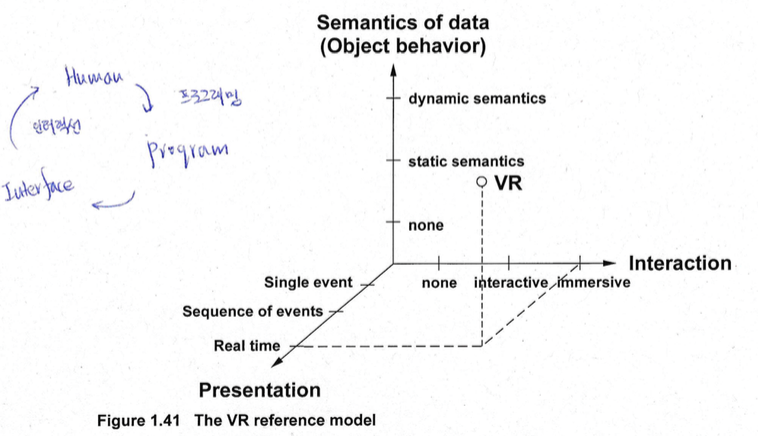
\includegraphics[width=\linewidth]{1_41}
\end{figure}

\subsubsection*{I$^3$ - Immersion - Interaction - Imagination}

\begin{itemize}
	\item technology provided by VR ...
		\begin{itemize}
			\item is used to immerse into the virtual env. (immersion)
			\item is used to interact with its objects. (interaction)
			\\ $\rightarrow$ VR addresses all perception channels of the user and thus he is convinced of the reality of VR env. (imagination)
		\end{itemize}
	\item i.e. Two prerequisites for VR: immersion \& interaction (\textbf{immersion \& interaction} $\rightarrow$ imagination)
	\item \textbf{latency time should be smaller than 0.1 sec!}
\end{itemize}

\begin{figure}[H]
	\centering
	\begin{subfigure}[b]{0.45\textwidth}	
		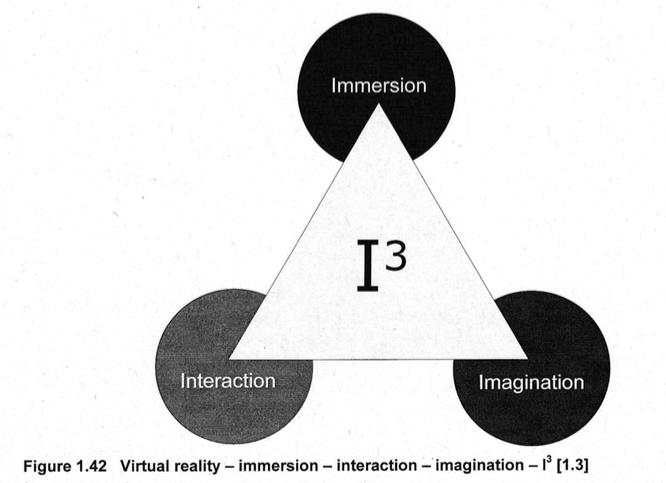
\includegraphics[width=\linewidth]{1_42}
	\end{subfigure}
	\begin{subfigure}[b]{0.45\textwidth}	
		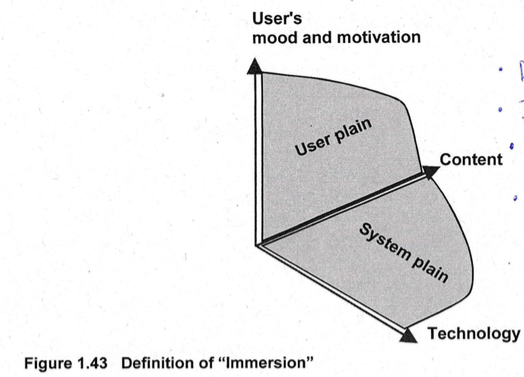
\includegraphics[width=\linewidth]{1_43}
	\end{subfigure}
\end{figure}

\subsubsection*{Interaction}

\begin{itemize}
	\item \textbf{interplay of information, action and reaction.}
	\item describes the effect of computer generated models onto the \textbf{human perception channels.} 
	\item continuous: continuous interaction with the virtual environment \textbf{(low delay)}
	\item reaction: every movement of the user causes a reaction in VR (note: difference with movies)
	\item generation / modification of geometry displayed, visual, acoustic, haptic, olfactory, and physical properties (e.g. collision, material prop., torque, DOF ...)of virtual object (copy or supplement real object)
	\item interactivity: ability of the system to allow a user's interaction, while the application is running. Special hardwares are needed.
	\item interaction facility 
		\begin{itemize}
			\item Passive: the user sees, hears and feel. (e.g. "Back to the Future" ride of Universal Studios)
			\item Exploratory: the user can explore the virtual env. 
			\item Interactive: the user explores the env, and interacts with the virtual objects also modify the env.
		\end{itemize}
\end{itemize}

\subsubsection*{Immersion}

\begin{itemize}
	\item Goal: to create the \textbf{``Sense of Presence" (SOP)} i.e. subjective impression of the user to be integrated in a fictive environment, which is not physically present.
	\item SOP focusing on...
		\begin{itemize}
			\item Natural interaction
			\item Interface to the computer is in the background
			\item Higher information density is possible
			\item More efficient access to complex data
		\end{itemize}
	\item User plain vs. System plain: interaction of both plains is the main purpose of supporting tech. Immersion is to map both plains onto each other.
\end{itemize}

\subsubsection*{Virtual Environment}

\begin{itemize}
	\item for interactivity, powerful computers are needed.
	\item sub-categories of virtual env.
		\begin{itemize}
			\item Reality driven virtual env.: generated model could also exist in reality
			\item Scaled virtual env.: computer generated which exists in reality, but can only be understood and explained by the user who applies the virtual model.
			\item Distant virtual env.: computer generated which represent a model of the real would cannot be explored out of distance or security reasons.
			\item Imaginative virtual env.: computer generated only come from the user's imagination.
			\item Informative virtual env.: visualize abstract data.
		\end{itemize}
	\item another sub-categories of virtual env.
		\begin{itemize}
			\item desktop virtual env.
			\item immersive virtual env.
			\item augmented virtual env.
			\item telepresence virtual env.
		\end{itemize}
\end{itemize}

\begin{figure}[H]
	\centering
	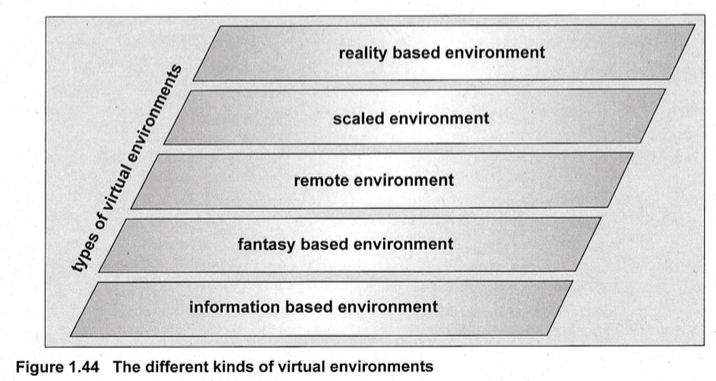
\includegraphics[width=0.6\linewidth]{1_44}
\end{figure}

\subsubsection*{Summary}

Virtual (VR) is a computer fictive world, which is characterized by the fact, that it can address \textbf{the perception channels} of the human user via interfaces. The user registers these sensations and answers by certain \textbf{reactions}. These reactions are registered by \textbf{the virtual environment} and cause corresponding reactions of the system. In order to complete the illusion of a new virtual reality, \textbf{only sensations from VR and not from reality can reach the user.} Thus, the user feels \textbf{completely immersed} in the virtual environment, which temporarily replaces reality. VR has to respond \textbf{fast and correctly} (corresponding to the defined rules) to the actions of the user.

\subsubsection{The Benefit of VR for industry}

\begin{figure}[H]
	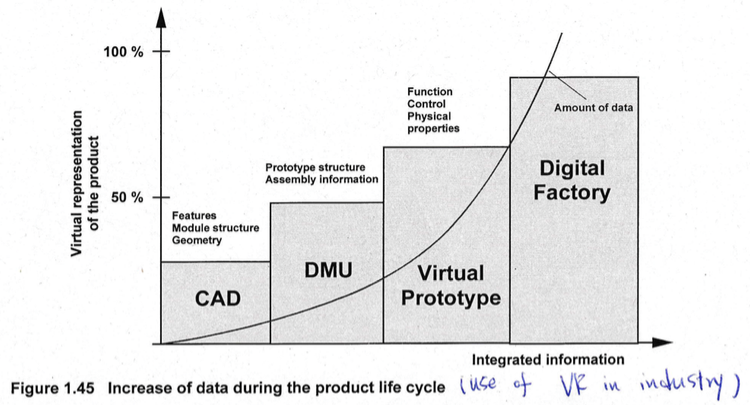
\includegraphics[width=\linewidth]{1_45}
\end{figure}

\begin{itemize}
	\item complexity of today's product $\rightarrow$ huge amount of data.
	\item product life cycle vs. data
		\begin{itemize}
			\item CAD: module geometry
			\item DMU(Digital Mock-up): assembly verification, collision detection and tolerance analysis
			\item Virtual prototype: physical properties (function simulation and software simulation)
			\item Digital factory: design and manufacturing process are considered
		\end{itemize}
	\item prototyping process up to now (physical mock-up)
		\begin{itemize}
			\item Digital proto $\rightarrow$ geometrical proto $\rightarrow$ functional proto $\rightarrow$ technical proto
		\end{itemize}
	\item now, VR is used for prototyping by DMU. (alternative of physical mock-up)
		\begin{itemize}
			\item \textbf{reach same quality of product in less time.} (Figure 1.47)
			\item \textbf{design modification iteration is much smaller and faster}: time \& cost-saving \\
				$\rightarrow$ much closer to ideal development process (Figure 1.48 and 1.49)
			\item all digital data gathered can be used later for other purposes (e.g. for the sales process)
			\item visualization of data: creative teamwork (idea generation)
		\end{itemize}
\end{itemize}

\begin{figure}[H]
	\centering
	\begin{subfigure}[b]{0.3\textwidth}	
		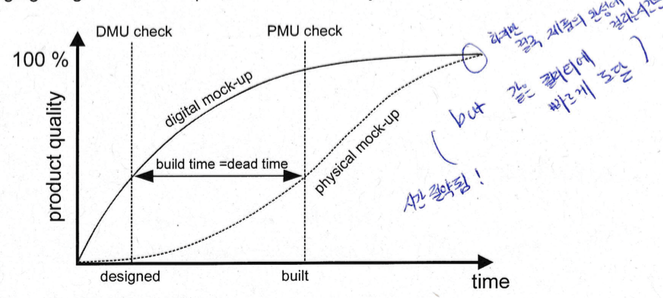
\includegraphics[width=\linewidth]{1_47}
	\end{subfigure}
	\begin{subfigure}[b]{0.3\textwidth}	
		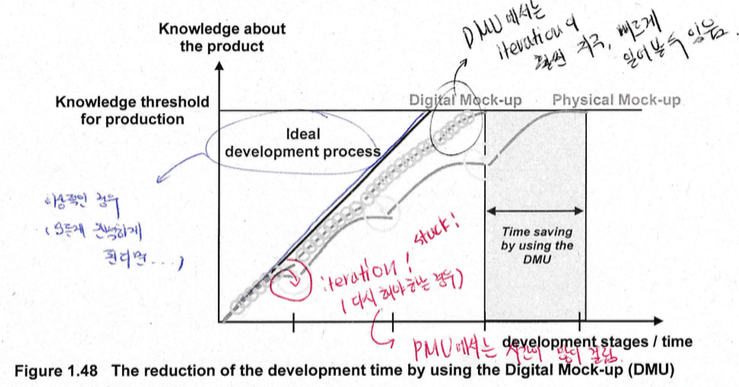
\includegraphics[width=\linewidth]{1_48}
	\end{subfigure}
	\begin{subfigure}[b]{0.3\textwidth}	
		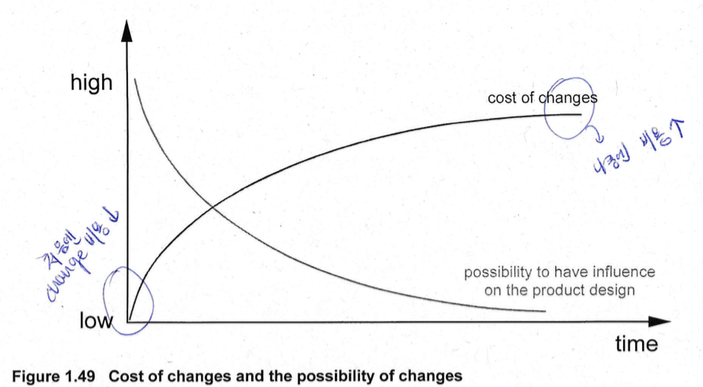
\includegraphics[width=\linewidth]{1_49}
	\end{subfigure}
\end{figure}

\subsubsection*{VR in product development process}

\begin{itemize}
	\item FMEA (Failure Mode and Effectiveness Analysis): visualization of geometry $\rightarrow$ detect possible failures, show the required details to all persons simultaneously.
	\item Access control: check accessibility to important point. (e.g. screw connections, connectors...: Figure 1.51)
	\item Kinematic verification: collision check w/o building (physical) proto.
	\item Design review: general design review. (geometrical proto)
	\item Crash simulation: automotive sector. Deformation process can be visualized.  
\end{itemize}

\subsubsection*{VR in Later production phases}

\begin{itemize}
	\item User training: for complex products, person can handle the product have to be taught in parallel. (e.g. escape from the plant in emergency)
	\item Product presentation: important part of the sales process. (e.g. Motor show)
	\item Assembly/service instruction: VR offers techniques and algorithms, which can drastically reduce the amount of data for complex geometries. (less powerful computer for visualization can be used.)
\end{itemize}

\subsubsection*{Digital product and services for user}

\begin{itemize}
	\item the structures of the digital product are optimized for the computer, not for the access by the user directly. 
	\item improvement of the interaction between the user and the digital product is a main requirement
	\item The user uses special \textbf{services} that allow him the access to the processes based on the digital product:
		\begin{itemize}
			\item visualize: content of the digital product or parts of it are visualized to the user. (graphical / text-based)
			\item simulate: unknown behavior will be simulated
			\item archive: all data about the product allows having instantaneous access to them
			\item document: documentation of a product or the processes (graphical / text-based)
			\item transfer: content of the digital product or excerpts of it are transferred over a network in a digital form
			\item present: excerpts of the digital product were extracted, processed and displayed. (optical aspects are in the focus of interest)
			\item integrate: excerpts of the digital product are integrated into the database. 
		\end{itemize}
\end{itemize}

\begin{figure}[H]
	\centering
	\begin{subfigure}[b]{0.45\textwidth}	
		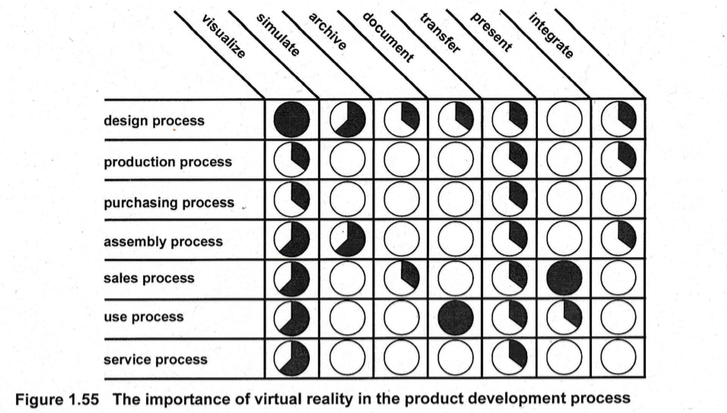
\includegraphics[width=\linewidth]{1_55}
	\end{subfigure}
	\begin{subfigure}[b]{0.45\textwidth}	
		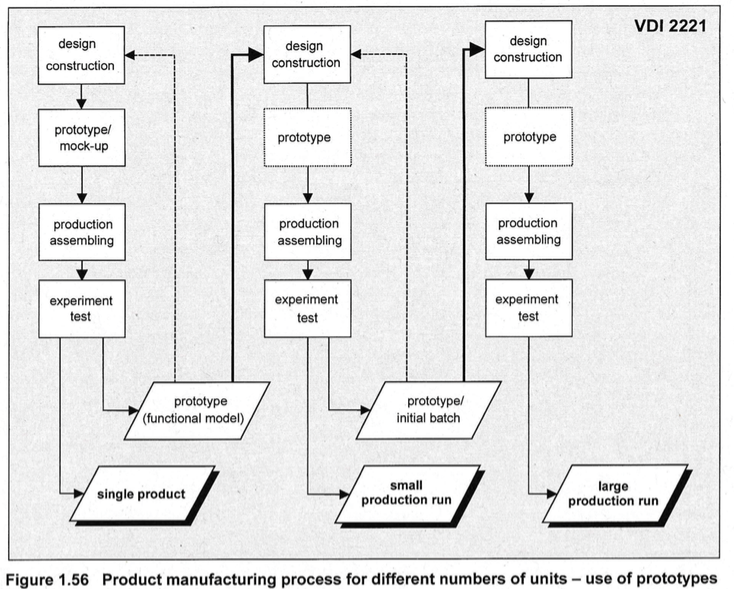
\includegraphics[width=\linewidth]{1_56}
	\end{subfigure}
\end{figure}


\subsubsection*{Real Prototypes and Mock-ups}

\begin{itemize}
	\item It is usual to pass the process several times and to create functional prototypes and initial batches.
	\item Benefit of using digital mock-ups (e.g. CAD, CAE)
		\begin{itemize}
			\item Communication: team works (e.g. marketing team $\leftrightarrow$ designer $\leftrightarrow$ process engineer)
			\item Documentation of the state-of-the-art: review the state-of-the-art of the product under development. (know-how reached so far and reduces uncertainties)
			\item Integration platform: integration of sub-systems. 
			\item Documentation of development steps (milestones): this can ensure the overall development goal can be achieved within a realistic time. 
		\end{itemize}
	\item New visualization technologies is to replace the physical proto. 
	\item VR allows the generation of synthetical environments in the computer for a realistic simulation of a design or construction.
	\item Digital mock-ups is in the dramatic reduction of development time, the higher product quality, and the reduction of cost for changes.
\end{itemize}

\begin{itemize}
	\item Note: classification of prototypes
		\begin{itemize}
			\item design proto: verification of the conceptual design concerning optical, esthetical, ergonomic requirements (not mechanical properties)
			\item geometrical proto: verification of dimensional, tolerances, and fits. (not material)
			\item functional proto: verification of mechanical, electrical, acoustical properties.
			\item technical proto: all functional. 
		\end{itemize}
\end{itemize}



\subsubsection*{Usage of VR and AR in the product development process}

\begin{itemize}
	\item VR - mainly at the beginning of the product's life cycle
	\item AR - increasing importance in the later stages 
	\item (the amount of VR decreasing) = (the amount of AR increasing)
	\item Note: at the present time, VR is a slight dominance. It's difficult to synchronize the real and the virtual object in time and position. (AR is much challenging)
\end{itemize}

\begin{figure}[H]
	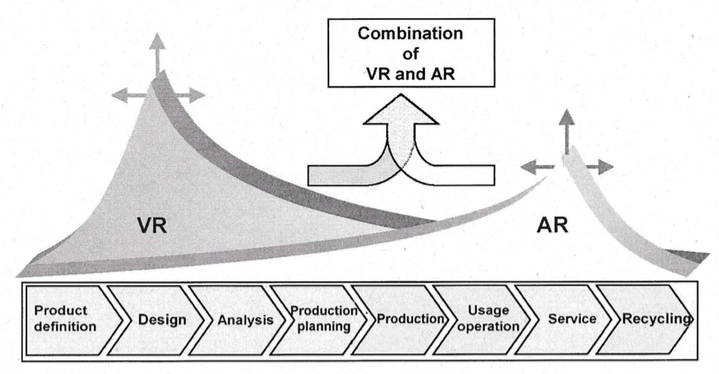
\includegraphics[width=\linewidth]{1_59}
\end{figure}

\end{document}
%\documentclass{standalone}
\begin{document}
\section{Chapter 2 Human Factors}
\begin{itemize}
	\item The goal is to stimulate all perception channels in such a way that the user feels completely immersed in the virtual environment and accepts it as real.
	\item visual, accoustic thermal, haptic and olfactory perception($80 \%$ of the overall information is perceived via the visual channel)
	\item Human Perception
	\begin{itemize}
		\item Perception
		\begin{itemize}
			\item Sensous physiology: the perception of stimuli, performed by sensory cells or by sensory organs.
			\item Psychology : Process of sensuous perception of an object without any conscious identification of the perceived object.
		\end{itemize}
		\item Psychology
		\begin{itemize}
			\item Psychology : Collective name for all processes or structures that are involved in the cognition process. e.g. imagination, estimation, mnemory, rememberance, learning. etc
		\end{itemize}
	\end{itemize}
	\item Four elementary attributes of stimulus
	\begin{itemize}
		\item modality: quality of a stimulus(the type of physical energy that is responsible for the stimulus)
		\item intensity: The strength of a stimulus defines the intensity of a sensation(below a specific threshold, the stimulus is not detected
		\item duration: relationship between the intensity of the stimulus and the duration of the sensation defines the perceived intensity
		\item location: The ability to locate the position of a stimulus and the ability to distinguish between two spatially close stimuli are important measures of the awareness of the spatial distribution of a sensory experience
	\end{itemize}
	\item only the sensory part of the cognition process can be addressed by devices of the virtual environment. (Figure)
\end{itemize}
\begin{figure}[H]
\centering
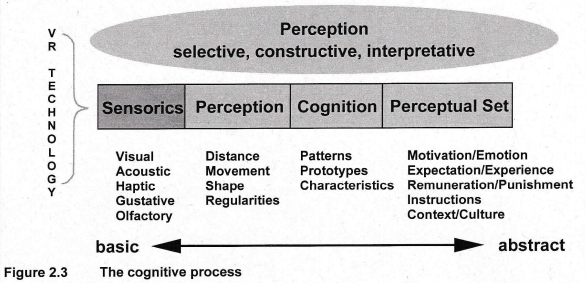
\includegraphics[width = 0.7\linewidth]{Figures/2_3.png}
\end{figure}
\subsection{The Human Eye}
\subsubsection{Viewing Angle}
\begin{itemize}
	\item Field of view characterized by: optical setup of the eye / the position of the eye in the face
	\item although field of view is very large perception of sharp images only possible in much smaller area
	\item viewing cones of both eyes overlap in a reange of approximately 120 degrees
	\item Four opening angles of the field of view
\begin{table}[H]
\centering
\begin{tabular}{|l|c|c|r|}
\hline
 nasal & temporal & superior & inferior \\ \hline
60 deg & 100 deg & 60 deg & 70 deg \\ \hline
\end{tabular}
\end{table}
\end{itemize}
\subsubsection{Temporal Resolution}
\begin{itemize}
	\item pupil can adapt to changing light conditions with a maximum frequency of 4 Hz	
	\item flicker consolidation frequency: maximum possible frequency without noticing any flickering
	\item perception of flickering not only depends on brightness but also the size of field of view and the location of light source it the FOV
\end{itemize}
\subsubsection{Accommodation and Convergence}
\begin{itemize}
	\item eye focuses onto shortest possible distance until object is visible: needs edges, patterns or contrours to focus: In compelte darkness, the eye cannot focus anymore
	\item results in near sightedness when looking through a optical device
	\item depth estimation up to 10 meters is made with stereoscopic vision $$ tan \frac{\epsilon}{2} = \frac{a}{2} \frac{1}{e}$$
\end{itemize}
\subsubsection{The Eye - Principle Set-up}
\begin{itemize}
	\begin{figure}[H]
	\centering
	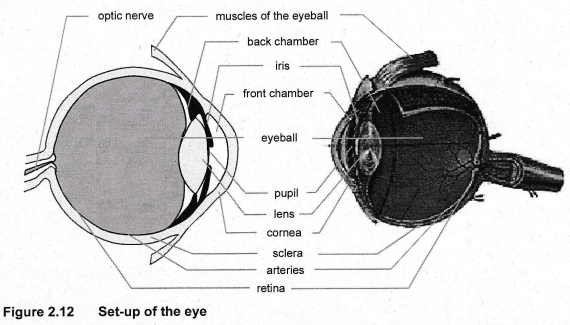
\includegraphics[width = 0.7\linewidth]{Figures/2_12.png}
	\end{figure}
\item eyeball has almost the shape of a sphere. Its skin consists of three layers: the outer sclera, athe arteries, and the retina
\item Light goes through the eyeball onto the retina
\item Retina consists of light receptors called uvulas and sticks which convert incoming light into electrical impulses
\item lens
\begin{itemize}
\item lens focuses the object onto the retina by adapting their focal length to the distance of the object
\item lens is fixed by fibers to the ciliar muscle. Activating or deactivating the muscle can change the geometry of the lens and thus the refraction
\end{itemize}
\end{itemize}
\subsubsection{B/W Perception, Color Perception}
\begin{itemize}
	\item light models: wave-model is more sufficient regarding the light as a electromagnetic radiation with a wavelength between 380nm and 780 nm
	\item color perception is done by a single eye
	\item color is perceived using special receptors on the retina
	\begin{itemize}
		\item sticks : only measure the intensity of the incoming light(Black and White). used at night but easily saturated.
		\item uvulas : used in daylight(light at night are not sufficient to work for uvulas), different uvulas for each color : (blue-sensitive uvulas 4 \% at 430nm , green-sensitive uvulas 32 \% at 530 nm, red sensitive uvulas 64 \% at 560 nm)
	\end{itemize}
	\item colors are coded into three basic colors, then two difference channels (red - green), (blue - yellow). addition of all colors result in the non-colored brightness.
		\begin{figure}[H]
			\centering
			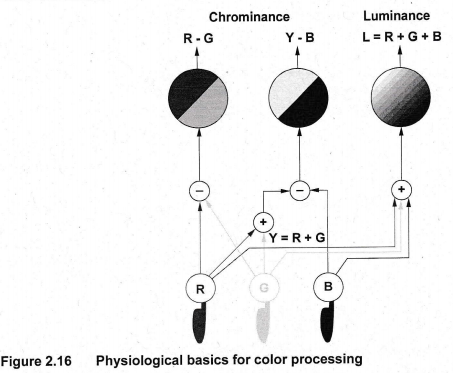
\includegraphics[width = 0.5\linewidth]{Figures/2_16.png}
		\end{figure}
\item During daylight: different kind of uvulas capture the basic colors red, green and blue while the sticks only measure brightness
\item During darkness: uvulas do not provide any color information, but only black(black does give any information to the brain?), small amount of light is sufficient to activate the sticks without saturating them
\item hue, saturation, brightness imitate the human color perception
\item there is also a contrast amplification in oerder to increase the perceived sharpness of the image
\item focal length depends on the color(Chromosteropsis: if more colors exist at the same distance, the eye can only focus on them, if red, blue exist the eye will focus on the red field due to the larger amount of red sensitive receptors)
\end{itemize}
\subsubsection*{Color Models}
\begin{itemize}
		\item CIE color model(Commission Internationale del'Eclairage): based on the typical sensitivity of the different uvulas(perception oriented color model)
		\item YUV color model: Takes into account the high green sensitivity into account, while sensitivity to red and blue is significantly lower(perception oriented color model)
		$$ C_b = B - Y color difference signal 1 \\
		C_r = R - Y color difference signal 2 \\
		Y brightness (luminance) $$
		\item RGB color model: does not take the physiology of the human eye into account(technical color model), basic colors are scaled to 1 and define a coordinate system
		\item CMY color model: is used by objects that do not emit light themselves, color used by printers
		\item HSV color model(also HSB): Defined by hue, saturation, value. In this color model, colors are arranged in a circle around the vertical axis
\end{itemize}
\subsubsection{Three-dimensional Viewing}
\subsubsection*{Spatial Viewing}
\begin{itemize}
\item spatial viewing can be performed with only one eye and thus is also called monocular viewing(only physiological aspects)
	\begin{itemize}
		\item Size of the Image on the Retina: If the real size is known, the brain compares the perceived size with the real size stored in the brain and calculates information of the position and the distance of the object
		\item Resoultion of the Perceived Image: Objects with blurred surface appear far away
		\item Overlap: If one object is in front of the other it has to be closer to the spectator than the object
		\item perspective: Far objects appear smaller than close ones
		\item shaded objects and shadows: I the light source is know, the object that causes the shadow appears closer to the light source
		\item textures: A spatial effect also appears when mapping textures perspectively onto an object. Wrong selection of textures could completely camouflage the geometry or pretend a wrong geometry
		\item motion parallax: the farther away an object is, the slower it moves on the retina when moving relatively to the user
	\end{itemize}
	\item Perception Rules Depending on geometry
	\begin{itemize}
		\item Rules of proximity: Spatially or temporally neighboring elements are perceived to belong together and to be part of the same element
		\begin{figure}[H]
			\centering
			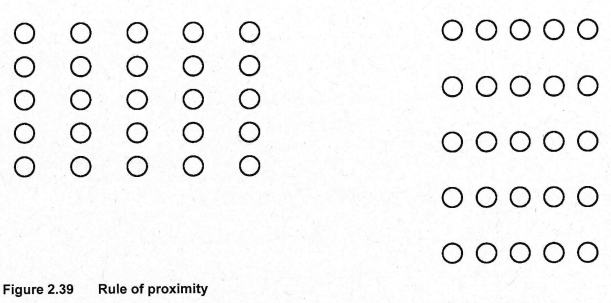
\includegraphics[width = 0.5\linewidth]{Figures/2_39.png}
		\end{figure}
		\item rule of similarity/rule of identity: Similar or identical objects appear coherently 
		\begin{figure}[H]
			\centering
			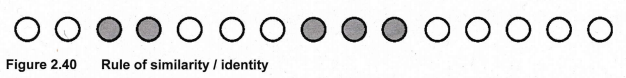
\includegraphics[width = 0.5\linewidth]{Figures/2_40.png}
		\end{figure}
		\item identity versus proximity: effects can be amplified or reduced
		\begin{figure}[H]
			\centering
			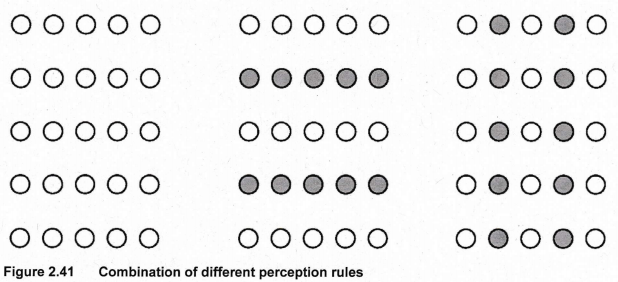
\includegraphics[width = 0.5\linewidth]{Figures/2_41.png}
		\end{figure}
		\item rule of harmonic continuation: elements that are spatially or temporally arranged in a simple harmonic or well defined order appear coherently and thus belong to the same geometric figure
		\begin{figure}[H]
			\centering
			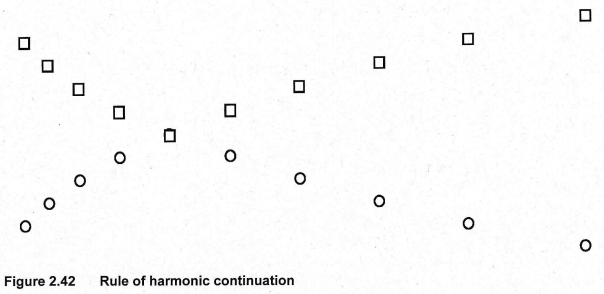
\includegraphics[width = 0.5\linewidth]{Figures/2_42.png}
		\end{figure}
		\item rule of closed lines: Contours, which are not completely closed, will be automatically closed during the perception process
			\begin{figure}[H]
				\centering
				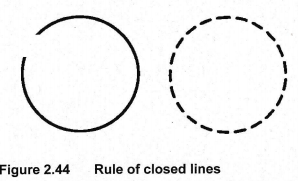
\includegraphics[width = 0.5\linewidth]{Figures/2_44.png}
				\end{figure}
		\item rule of symmetry: if none of the mentioned rules could be applied, the space between symmetric contours shapes a figure, rather than the space between asymmetric contours
			\begin{figure}[H]
				\centering
				
\includegraphics[width = 0.5\linewidth]{Figures/2_45.png}
			\end{figure}
		\item the principle of harmonic shape: The structure will be perceived, that has as many simple figures as possible
			\begin{figure}[H]
			\centering
			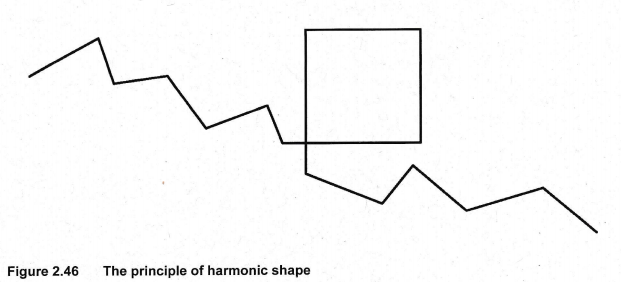
\includegraphics[width = 0.5\linewidth]{Figures/2_46.png}
			\end{figure}
		\item contours: 
			\begin{figure}[H]
			\centering
			
\includegraphics[width = 0.7\linewidth]{Figures/2_47.png}
			\end{figure}
	\end{itemize}
\end{itemize}
\subsubsection*{Allocation Problems}
\begin{itemize}
	\item wrong perspective, brightness of objects given context, comparison with known patterns
	\item peripheral drift illusion: depends on difference in brightness or color
	\item Hermann grid: Different structures of receptive areas can be realized by individual interconnections
		\begin{figure}[H]
			\centering
			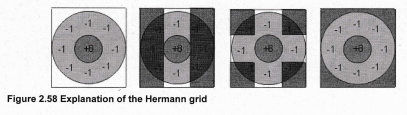
\includegraphics[width = 0.7\linewidth]{Figures/2_58.png}
		\end{figure}
\end{itemize}
\subsubsection*{Stereoscopic viewing}
\begin{itemize}
	\item The point is projected on non-corresponding areas on the retina on both eyes. This gives a spatcial impression
\end{itemize}
\subsubsection{Conflicts between Virtual Reality and the Physiological and Psychological Visual Perception}
\begin{itemize}
	\item Since all virtual objects are visible on the projection plane, the human eye does not have to perform an accommodation anymore, but only focuses once on the given distance between the user and the projection plane
	\item psychological apsects are also not fulfilled
\end{itemize}
\subsection{The Human Ear}
\begin{itemize}
	\item Functionality of hearing
	\item Sound signals and sound sources
	\item Location of sound sources
	\item sensitivity and loudness(very important psychological factor)
\end{itemize}
\subsubsection{Anatomical Set-up of the Ear}
\begin{itemize}
	\item Human ear can be seprated into three, anatomically different organs
		\begin{itemize}
			\item outer ear: auricle and the auditory canal belong to the outer ear
			\item middle ear: a mechanical impedance converter is situated between the eardrum and the inner ear, consisting of three bones-hammer, anvil, stirrup
			\item inner ear: Consists of a spiral pipe, which gets thinner and is filled with fluid, the medium for acoustic wave dissemination is the air, while in the inner ear a fluid(lymph) is ued
		\end{itemize}
	\item sensitivity of the human ear is frequency dependent
	\item accoustic pressure level $L_p$ is a quantity that can be directly measured but not directly correspond to the subjective impression of loudness
	\begin{equation}
	L_p = 20 log \frac{p}{p_0} [dB]
	\end{equation}
	\item The complete field between the pain threshold and the accoustic threshold is called the perception area
\end{itemize}
\subsubsection{Spatial Hearing}
Spatial hearing desribes the accoustical determination of a sound source's position in a room. Two princilples:
\begin{itemize}
	\item monaural hearing
	\begin{itemize}
		\item Using one ear only: very rough localization($\pm 20 \deg deviation from correct localization$) : does not play important role
	\end{itemize}
	\item binaural hearing
	\begin{itemize}
		\item difference in intensity: only possible if wavelength of the sound is small compared to the size of the head
		\item difference in runtime: brain capable of detect runtime differences of approximately 30us
		\item can calculate the run time difference:
		$$
		\Delta x = d sin \alpha \\
		\Delta t = \frac{\Delta x}{c} = \frac{d}{c} sin \alpha \quad c = 340m/s
		$$
	\end{itemize}
	\item Sound and Tone
		\begin{itemize}
			\item A sound sensation, which has a periodic oscillation but a non-sinusoidal waveform can be generated by a superposition of multiple sinewaves with different amplitudes and frequencies(frequencies have to be in an integral relation ship with each other). All sound sensations that fulfill the requirement are also named a tone
		\end{itemize}
	\item Allocation Problems of the ear
			\begin{itemize}
			\item Shephard effect: simulates increasing melody to the user although the pitch stays constant all the time
		\end{itemize}
\end{itemize}
\subsection{The Haptic Channel}
\subsubsection{The Human Information Flow}
\begin{itemize}
	\item the entirety of all perceptions through the sense of touch
	\item about 80 \% of all information is perceived by the visual sense, other 15 \% by the auditory sense. The remaining 5 \% are fr the haptic and olfactoric sense. 
\end{itemize}
\subsubsection{The Haptic Perception}
\begin{itemize}
	\item The haptic takes place all over the body, thus it is impossible to generate a complete simulation in the haptic field: The human hand is the most relevant element in the field of haptics
	\item well known input device: mouse and keyboard provide haptic feedback addition to acoustic feedback.
	\item required for teleoperation
	\item Using the had to perform a manipulation
	\begin{itemize}
		\item Contact Phase: Describes the first contact of the fingers with an object(felt 200 ms after contact)
		\item Grasping Phase: has the largest flexibility and interactability
		- Grasping for increased power / Grasping with increased dexterity
		\item Touching Phase: For characterizing the properties of objects, different hand-object interactions are needed
	\end{itemize}
	\item Grasping can be seperated with thwo fields
	\begin{itemize}
		\item grasping with increased power
		\item grasping with increased dexterity
	\end{itemize}
	\item Haptic desribes the influence of foces of any kind onto the human body(tactile propriorceptive, kinesthetic)
	\begin{itemize}
		\item tactile: using perception cells in the skin(pressure, temperature, vibration)
		\item propriorceptive: Influence of force caused by the weight of the object onto the sensors in the musculature
		\item kinesthetic sensation is the perception of acceleration forces onto the body 
	\end{itemize}
\end{itemize}
\subsubsection*{Basics on the Physiology of the Senses in the Skin}
\begin{itemize}
	\item Skin registers pressure, touch, vibration (=sense of touch), temperature and pain. This surface sensibility (together with the depth sensibility (muscle, joint and string receptors)) is also called somatovisceral sensibility
	\begin{itemize}
		\item Meissner cells and hair receptors: detect the touch.(Not the intensity is important(bending of the hair) but the speed by the sensation changes.
		\item Pacini cells: specialized to detect vibrations
	\end{itemize}
	\item receptors can be divided into slowly adapting and rapdily apdapting mechanoreceptors
	\begin{itemize}
		\item rapidly adapting receptors respond to onset and often also termination but not throughout during stimulus-> sensorial adaptation
	\end{itemize}
	\item receptors can be classified by spatial resolution and temporal resolution
	\begin{itemize}
		\item intensity receptors: P-receptors
		\item speed receptors: D-receptors
		\item PD receptors are a mixture, which measure for example the position of the joints
	\end{itemize}
	\item Thermo receptors exist for a temperature range below 36 degrees
\end{itemize}
\subsubsection{Depth Sensibility; Distension Reflex}
\begin{itemize}
	\item proprioreceptors: for measuring the position of the joints, the length of the muscles etc(depth sensibility) so-called proprioceptors exist
\end{itemize}
\subsection{The collaboration of all Senses}
\begin{itemize}
	\item conscious and unconscious perception can be described using the so-called inner model
	\begin{itemize}
		\item Describes the context between the performed action and the expected sensor information
		\item the inner model contains the expected values of the receptors for the performed action
	\end{itemize}
	\item Pushing a button example
	\begin{figure}[H]
			\centering
			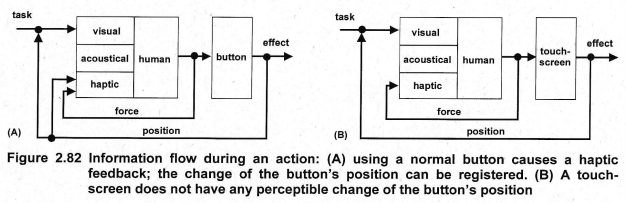
\includegraphics[width = 0.5\linewidth]{Figures/2_82.png}
	\end{figure}
	\item McGurk effect: If acoustic and visual stimuli are not correlated
\end{itemize}
\end{document}
%\documentclass{standalone}
% Load any packages needed for this document
\begin{document}

\section{Chapter 3: Introduction into Computer Graphics}

\subsection{Introduction}

\begin{itemize}
	\item Quick development in computer graphics: from an expensive toy to an attractive research field
		\begin{itemize}
			\item main reason: human receives most of the information through the visual perception channel
			\end{itemize}
	\item Rapid development concerning hardware, software, and applications
		\begin{itemize}
			\item graphics can be easily accessed and understood by different cultures/people/languages (high synergy among people)
		\end{itemize}
\end{itemize}

\subsection{Why do we need Computer Graphics?}

\begin{itemize}
	\item The representation of texts is also a special form of graphics
	\item Human being seems to have a better access to images and pictures than letters and numbers
		\begin{itemize}
			\item e.g. complex simulation results by visualization, logo of a company
		\end{itemize}
\end{itemize}

\subsubsection*{Computer Graphics and Picture Recognition}

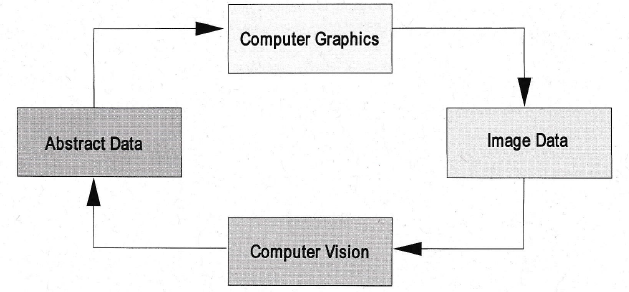
\includegraphics[scale=0.6]{3_1}

\begin{itemize}
	\item When a human perceives the surrounding world, the brain generates an abstract "data model"
	\item Computer Vision: extract relevant data out of existing graphics or images
	\item Computer Graphics: display the data
\end{itemize}

\subsection{Applications of Computer Graphics}

\subsubsection*{CAD}

\begin{itemize}
	\item Construction (Functional Design)
	\begin{itemize}
		\item the requirements to an assembly part are well defined by function and dimension
		\item all drawings on a CAD system are a complex relationship between dimensions, constraints, and material properties, which describe a part very well
	\end{itemize}
	\item Design (Aesthetic Design)
	\begin{itemize}
		\item do not focus on the dimension of a part, but factors like ergonomics or aesthetics
		\item many suppliers of design software try to combine the relatively free aesthetic design field with the very compulsory functional design, but hasn't been successful due to difficult exchange of data between both worlds
	\end{itemize}
\end{itemize}

\subsubsection*{Gaming}
\begin{itemize}
	\item Caused a significance increase of graphic performance in the private computer sector
	\item Cheap components and fast, high- quality software were developed due to the growing demands of players and the competition of the industry
\end{itemize}

\subsubsection*{Visualization}

\begin{itemize}
	\item Visualization is the ancestor of 3D computer graphics
	\item \textbf {Definition: Visualization addresses special properties of human perception to visualize and to represent information, which is extracted from large amount of data}
	\item Visualization intends to:
	\begin{itemize}
		\item display structures, models, trends, anomalies, and relationships
		\item give an overview of large amounts of data
		\item give support by means of an easy modification of parameters when searching for interesting regions in a large data field
	\end{itemize}
	These points can be summarized in the mantra of Ben-Shneiderman:
	\begin{center}
	\textbf{overview, zoom-in, filtering, details on request}
	\end{center}
	Thus, a good visualization has the following properties:
	\begin{itemize}
		\item it prevents misinterpretation and ambiguity
		\item it optimizes the perception of subtle properties
		\item it allows displaying more data at a time
	\end{itemize}
	\item Typical data sets which need to be visualized very often:
	\begin{itemize}
		\item MRI (the density can be visualized by different colors and transparencies)
		\item CFD (the location and the direction of movement of points with 6 DOF, color and particles, size or shape can display the information)
		\item Financial Data (display in a diagram, so that a user can see correlations between variables)
		\item CAD (3D data with additional information for edges, corners, surfaces, and surface properties. Complex data structures are used because the data is used not only for visualization but also for other processes. Complexity of the models strongly depends on the display quality)
		\item Statistical data sets (the correlation between different parameters only can be seen through visualization)
	\end{itemize}
	\item Different kinds of visualization in the following table. The different categories do overlap in many cases, "Illustration" has an exceptional position since it can be used everywhere
\end{itemize}

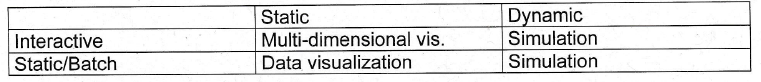
\includegraphics[scale=0.7]{3_8}

\begin{itemize}
	\item Data Visualization
		\begin{itemize}
			\item The most common way would be Excel-like presentation (e.g. pancake diagram, 3D graphs)
		\end{itemize}
	\item Cybernetic Visualization (Simulation)
		\begin{itemize}
			\item The main interest in the visualization of a cybernetic application: speed and possible detection of errors and irregular behavior of the simulated system
			\item The classical way: showing data in a 2D graph as a time-dependent value
		\end{itemize}
	\item Multi-dimensional Visualization
		\begin{itemize}
			\item when much data has to be displayed simultaneously within one image
			\item every point in the space can represent 3 independent values + color, line thickness, transparency, different shapes, etc.
			\item other ways exist but a compromise has to be made concerning the simplicity (e.g. switch between different data visualization planes on any given point of a curve or shape)
		\end{itemize}
	\item Statistics
		\begin{itemize}
			\item typically statistics contain many different values for one single measurement.
			\item the visualization's task is showing possible correlations among the different values
			\item only valid for the given constraints
		\end{itemize}
\end{itemize}

\subsubsection*{Illustration}

\begin{itemize}
	\item Illustrations are 2D add-ons to a 3D object. They contain much additional information about the 3D representation.
	\item GUIs
		\begin{itemize}
			\item the most important means of communication between the user and the computer
			\item the most important input device is the mouse
			\item basic idea of GUI: pointing on an object is one of the easiest gestures of a human being
			\item within the GUI an icon is a small image, which is a representation for a program sequence or for the content of a defined type (they made working with a computer much faster and more comfortable because people can just 'click' on them instead of entering complex instructions)
		\end{itemize}
	\item Fonts
		\begin{itemize}
			\item within the visualization, text is used to assign abstract contents like titles, classifications, or dimensions to a graphical object
			\item Typesets and fonts are the medium of text (based on typography and applications)
		\end{itemize}
	\item Layout
		\begin{itemize}
			\item By placing graphical elements on a surface, the underlying information is structured more clearly and more detailed
			\item typical applications: windows-based desktops such as MacOS, Windows (e.g. word wrap)
			\item Another kind of layout is characterized by the given application (e.g. simulation of operation elements in a car- the ergonomic placement of the elements is essential for the overall handling of the vehicle)
		\end{itemize}
	\item Drawings
		\begin{itemize}
			\item very often used to visualize abstract situations
			\item e.g. organization charts or flowcharts, manuals
		\end{itemize}
	\item Instructions
		\begin{itemize}
			\item instructions consist of a mixture of text, graphical visualization, photos, etc.
			\item very often they visualize products in an abstract and simplified way
			\item e.g. service manuals, assembly manuals
		\end{itemize}
\end{itemize}

\subsection{Definition of 3D Graphics}

\begin{itemize}
	\item Definition of 3D graphics: \textbf{The field 3D graphics deals with the generation of 3D objects and their representation on a two-dimensional surface(e.g. a screen)}
	\item the main focus is on projection and visualization of a 3D space on a 2D surface of any kind
	\item example of 3D graphic devices: video camera, photo camera
	\item main characteristics of 3D graphics:
	\begin{itemize}
		\item data acquisition / data transfer / storage
		\item transformation / processing
		\item data display on 2D
		\item input and output
	\end{itemize}
	\item simple pipeline for data processing: \\
		$\rightarrow$ Definition of geometry as digital data \\
		$\rightarrow$ Processing and transformation of data \\
		$\rightarrow$ Transformation of data to 2D \\
		$\rightarrow$ Display of the results on a screen
\end{itemize}

\subsection{Rendering Pipeline}

\begin{itemize}
	\item The rendering pipeline is the basis for almost every application in computer graphics
	(can be slightly modified for special applications such as augmented reality)
	\item The simplest form of the rendering pipeline: \\
	$\rightarrow$ Processing and transformation of data \\
	$\rightarrow$ Transformation of data to 2D \\
	$\rightarrow$ Display of the results on a screen
	\item transformation / processing: modify the original data in such a way that it can be displayed well on a 2D surface. contains data modified by the user e.g. modified viewing angle onto the geometry
	\item transformation of data to 2D: all modified data has to be transformed onto the 2D surface. e.g. removal of hidden objects or surfaces, transferring a curved surface into triangles, or the integration of illumination models
	\item input/output: reduce the amount of data so that the image can be optimally displayed on the output device (due to limitation in resolution)
\end{itemize}

\subsection{Definition of Geometry in the Computer}

\begin{itemize}
	\item Algorithms for a geometric representation of curves and bodies were developed in order to model hulls, car bodies, and fuselages
	\item B\'ezier developed a CAD-system (further developed into the 'UNISURF' system later on), close approximation to geometry
	\item In order to define geometry, the information should be sufficient but not redundant
	\item It can be distinguished between volumetric and surface models
\end{itemize}

\subsubsection*{Discrete Definition of Surfaces}
\begin{itemize}
	\item Cloud of Points:
	\begin{itemize}
		\item the simplest model, every point of the cloud is defined by its coordinates
		\item The point cannot be rendered(no information on color or texture) and there is no connectivity among the points(separate parts cannot be selected in the model)
		\item 3D-scanner typically provides a cloud of points
		\item difficult to create a good surface out of the clouds of points because the acquired data is noisy and erroneous
	\end{itemize}
	\item Polygons, Tessellation:
	\begin{itemize}
		\item Tessellation is a method for defining or generating a mesh of geometric basic elements(polygons), which approximate a complex surface
		\item Polygon, especially triangle, is one of the most important basic elements of computer graphics
		\item "triangulation": the process in which a free-form surface is transformed into triangles (The mesh approximates the surface by triangles and reduces the complexity)
		\item additional data has to be considered when rendering (e.g. perpendicular of a surface)
	\end{itemize}
	\item Polystrips
	\begin{itemize}
		\item when a point is added to a triangle, a second triangle will be generated
		\item advantage: a large amount of surfaces can be generated by a very low amount of data
		\item stored in two tables: the point(vertex) table with all coordinates of the triangle's corners and the strip table with all coherent triangles
		\item details could be lost since any curve is approximated by straight lines of different lengths
		\item many times the triangulation is done at a very late stage in rendering because often working with mathematically exact representations of the geometry is required
	\end{itemize}
\end{itemize}

\subsubsection*{Mathematical Description of Geometries}

\begin{itemize}
	\item Typically, the surfaces of objects are represented by approximating functions
	\item A parametric representation is used for the approximation or interpolation of these surfaces (e.g. parametric polynomials - B\'ezier, B-Spline)
	\item Surface models are mainly used- drawback: there are no relationships among the individual parts of the surface (The individual surfaces are not correlated with an object and thus the shape of an object is a question of interpretation)
	\item possibilities for the mathematical description of curves and surfaces: explicit, implicit, parametric
	\begin{itemize}
		\item explicit: only one value for y is associated with the variable x\\
		thus problems arise for closed curves or objects\\
		it is not invariant to rotations\\
		only a few geometries can be described by such an explicit notation, rarely used
		\item implicit: typically implicit equations have more solutions than required and thus additional constraints have to be considered\\
		also rarely used in virtual reality
		\item parametric: the most common descriptive form\\
		no equivocations could occur, the definition is invariant to rotations\\
		infinite slopes can be described by tangential vectors which are finite\\
		typically consist of rational polynomials of the nth degree, most frequently cubic polynomials are used\\
		any point of the geometry can be exactly determined by mathematical functions (particular interest for CAD)
	\end{itemize}
	\item B\'ezier splines:
	\begin{itemize}
		\item first used in shipyards
		\item goal: interconnect given points by a smooth line
		\item points that approximate the curve are called "control points"
		\item mathematical function that delivers the result is named "base function", guarantees that the requirement for continuity in the control points is kept by interpolation or approximation
	\end{itemize}
	\item approximation: a curve approximates given control points / interpolation: the calculated curve has to meet the control points exactly; important in both cases that continuity is fulfilled
	\item "parametric continuity":
	\begin{itemize}
		\item represented by the letter C and its exponent i which defines the degree of the i\textsuperscript{th} derivation \\
		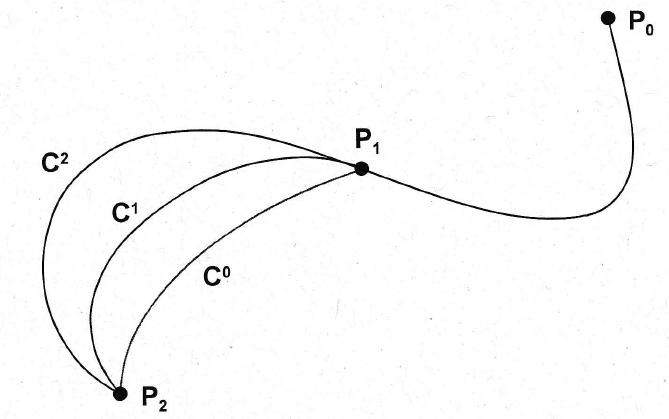
\includegraphics[scale=0.5]{3_24}
		\item C\textsuperscript{0} continuity: guarantees that the curve is not interrupted, but it could happen that a curve is not smooth in the point P1 but has an edge instead
		\item C\textsuperscript{1} continuity: the first derivation is continuous, all tangent vectors in the point P1 have the same slope, the curve is smooth at the point P1 (continuity of tangents)
		\item C\textsuperscript{2} continuity: the second derivation is continuous, the curve looks even smoother, also named as continuity of curvature
	\end{itemize}
\end{itemize}

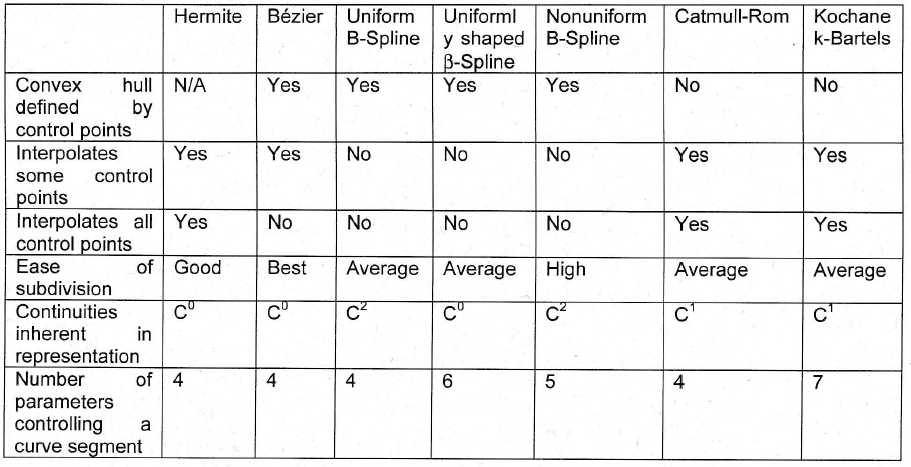
\includegraphics[scale=0.6]{3_25}

\subsubsection*{Approximating Splines}

\begin{itemize}
	\item If an approximating curve is described by control points, there is an additional requirement that the resulting curve has to be within the polygon shaped by the control points
	\item The shape is a complex polygon that encloses all control points like a rubber band
	\item If the control points are extreme points, they are part of the polygon; otherwise, they are inside of the polygon
	\item The complex shape allows a good control of the curve (guarantees the curve is always within the visible area)\\
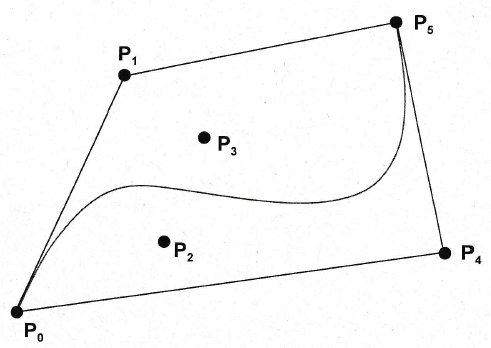
\includegraphics[scale=0.5]{3_26}
	\item B\'ezier Curve
	\begin{itemize}
		\item the base function is defined in a parametric form Q(t), t is a variable within [0, 1)
		\item the base function depends on the amount of control points; the whole curve is changed by just changing one point
		\item in addition to B\'ezier curve, also the first and last control point belong to the curve Q(t)
		\item always inside a complex polygon, because at least three control points are extreme points
		\item The Algorithm of de Casteljau: \\
		The base function of a B\'ezier curve can be calculated by the algorithm of de Casteljau\\
		idea: choose t and subdivide the first line b\textsubscript{0}b\textsubscript{1} at the distance t
		\begin{equation}
			b\textsubscript{0}\textsuperscript{1}(t) = (1-t)b\textsubscript{0}+t b\textsubscript{1}
		\end{equation}
		This process is repeated for the lines b\textsubscript{1}b\textsubscript{2} and b\textsubscript{2}b\textsubscript{3}, until in total three new points b\textsubscript{0}\textsuperscript{1}, b\textsubscript{1}\textsuperscript{1}, b\textsubscript{2}\textsuperscript{1} will result \\
		the calculation is repeated with the three new points and so on \\
		In general:
		\begin{equation}
			b\textsubscript{i}\textsuperscript{r}(t) = (1-t)b\textsubscript{i}\textsuperscript{r-1}+t b\textsubscript{i+1}\textsuperscript{r-1}
		\end{equation}
		\begin{equation}
			b\textsubscript{i}\textsuperscript{r}(t) = b\textsubscript{i}
		\end{equation}
		i = number of control points; i=0,...(n-r), r = number of lines; r=1,...,n
	\end{itemize}
	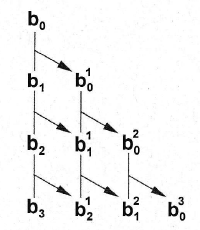
\includegraphics[scale=0.75]{3_29} 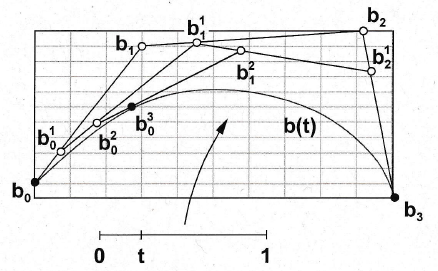
\includegraphics[scale=0.75]{3_30}
	\begin{itemize}
		\item For a better approximation of the curve, more control points have to be used which will increase the computing time
		\item The algorithm of de Castelijau can also be used, if more than four control points exist
		\item The number of control points(L+1) defines the kind of curve
		\item For L=3 (cubic B\'ezier curve), it is further elaborated and simplified as:
		\begin{equation}
			Q(t) = b\textsubscript{0}(1-t)\textsuperscript{3}+b\textsubscript{1}3t(1-t)\textsuperscript{2}+b\textsubscript{2}3t\textsuperscript{2}(1-t)+b\textsubscript{3}t\textsuperscript{3}
		\end{equation}
		\item Bernstein Polynomials: \\
		B\'ezier curves can be more easily calculated by using it; do not work recursively but directly deliver the result at the position t by using polynomial coefficients \\
		When (L+1) control points are given, the function is defined by:
		\begin{equation}
			Q(t) = \sum_{i=0}^Lb\textsubscript{i} B\textsubscript{i}\textsuperscript{L}(t)
		\end{equation}
		$$ B\textsubscript{i}\textsuperscript{L}(t) $$ is the Bernstein polynomial, which is defined as:
		\begin{equation}
			B\textsubscript{i}\textsuperscript{L}(t)= \textsubscript{L}C\textsubscript{i} (1-t)\textsuperscript{L-i}t\textsuperscript{i}, \quad L >=i
		\end{equation}
	\end{itemize}
	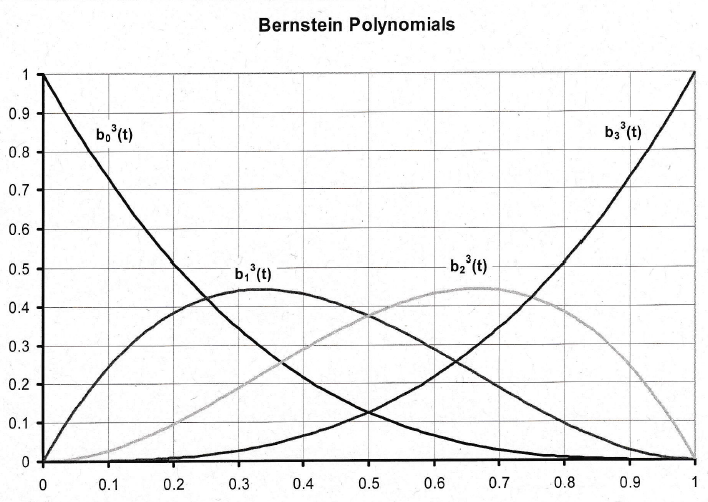
\includegraphics[scale=0.65]{3_31}
	\begin{itemize}
		\item If B\'ezier curves of a high degree are employed, it is difficult to keep the curve smooth
		\item Bernstein polynomials can also be calculated by a successive superposition of linear B\'ezier splines
	\end{itemize}
	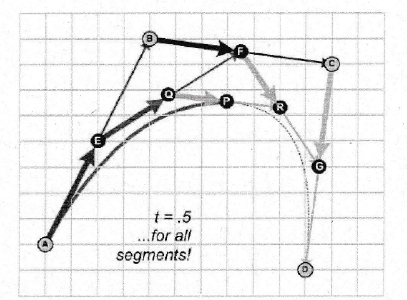
\includegraphics[scale=0.8]{3_32}
\end{itemize}

\subsubsection*{Interpolating Splines}

\begin{itemize}
	\item Boundary Representation - B-Rep
	\begin{itemize}
		\item Edge representations(or surface models or boundary representation) use 3D polygons to define the limiting surfaces of an object \\
		The limiting surfaces can be plain surfaces, but also surfaces of higher order \\
		It allows an exact mathematical description for many geometries, good approximation for the others
		\item B-Rep models consist of three object types: surfaces, edges, and corners
		\item To create on object out of the individual surfaces, the data structure must also contain a topological part(which defines the neighborhood of the surfaces) beside the normal geometric definition \\
		very common topological list contains 4 parts: a list of points/edges/surfaces/volumetric objects \\
		This list corresponds to a point-edge-surface model \\
		advantage: compact storage of all defining elements, since every point has to be stored only once
		\item The advantage of surface models consists in the complete availability of all topological information \\
		Surfaces, edges, and points can be stored as individual objects, which significantly increases the flexibility of the object \\
		one drawback: high calculation effort and complex network structure
	\end{itemize}
\end{itemize}

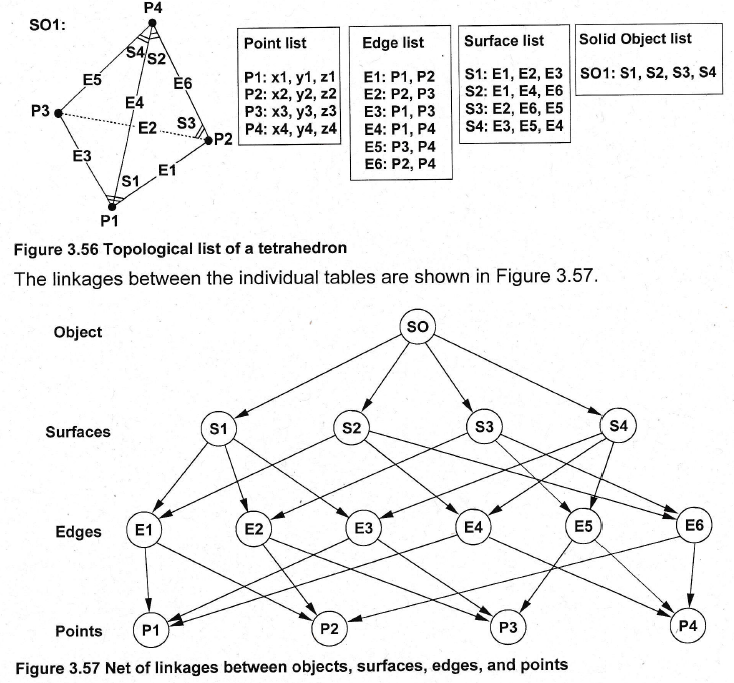
\includegraphics[scale=0.7]{3_56}

\subsubsection*{Volumetric Models}

\begin{itemize}
	\item The goal is to create objects that can be generally used (not only suitable for special applications)
	\item Only complete representations of physical objects are accepted
	\item Volumetric models can be distinguished into: \\
	cell models: these models discretize the required space of the object \\
	accumulative models: the object consists of a sum of basic elements \\
	generative objects: predefined volumetric elements (primitives) and Boolean operations on the elements \\
	other models: parametric models(e.g. CAD), sweep models, breakdown into elements(FEM)
	\item CSG(Constructive/Computational Solid Geometry)
	\begin{itemize}
		\item 3 primitive methods to shape geometry out of simple objects: merging parts(set union), cutting parts out(difference), calculate common parts of objects(intersection) $\rightarrow$ this approach is used by CSG
		\item CSG uses simple basic geometries like cones, spheres, cubes which are completely described by mathematical functions
		\item Complex objects can be described by a tree of Boolean operations		
	\end{itemize}
	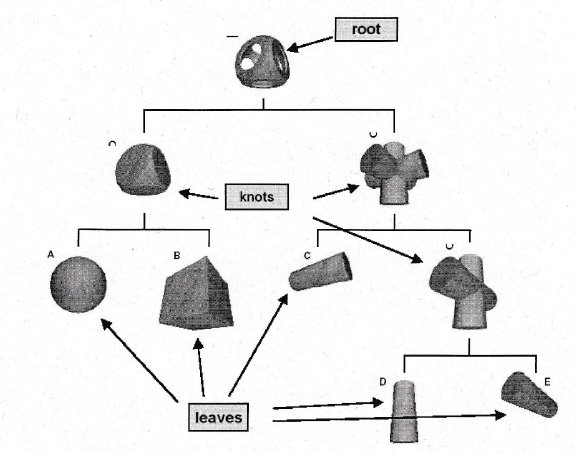
\includegraphics[scale=0.8]{3_62}
	\item Cell Models
	\begin{itemize}
		\item In analogy to pixel models, cell models use voxels(volume elements) of uniform size to represent volumetric models
		\item the voxels are arranged in a regular 3D grid and are represented by the coordinates of the cell's center
		\item the maximum resolution is defined by the cell size
		\item the representation of 3D objects using cell models is suitable for the computation of volumes and other Boolean operations; however the geometrical elements(corner, edge, surface) can only be represented imprecisely or with a large effort
	\end{itemize}
\end{itemize}

\subsection{Color Definitions in the Computer}

\subsubsection*{Color Depth and Color Palettes}

\begin{itemize}
	\item The maximum number of colors to be used by the computer is defined by the color depth, i.e. the amount of bits that describe a color
	\item (number of colors) = $2^{color depth}$ (e.g. color depth 1 means 2 colors can be used)
	\item If the color depth is smaller than 8 bits, color palettes(color look-up tables, LUT) are used
	\begin{itemize}
		\item color palettes: an array in which each entry defines exactly one color
		\item thus, this array contains color information for each pixel
	\end{itemize}
	\item In the picture memory, references to the LUT exist
	\begin{itemize}
		\item if colors change, the entry in the LUT is modified while the picture memory stays unchanged
	\end{itemize}
	\item Each entry in the look-up table consists of a tuple of numbers for the colors RGB
	\item If the color depth is larger then 8 bits, the color look-up table would become too large and thus color information is directly stored in the picture memory
\end{itemize}

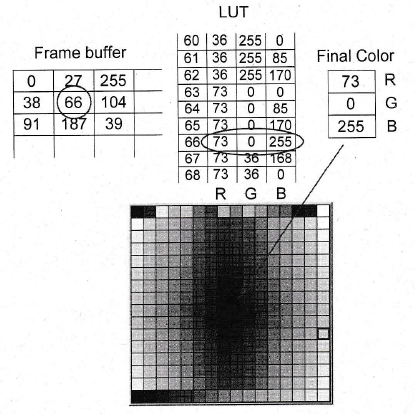
\includegraphics[scale=0.7]{3_64}

\subsubsection*{Color Quantization}

\begin{itemize}
	\item Color Quantization: to reduce the required memory for displaying images
	\begin{itemize}
		\item Due to the immense costs of memory chips, the available graphic memory was restricted for a long time
		\item Thus, old graphic cards could only display images with a color depth of 8 Bit with a poor resolution
		\item Images with a higher color depth had to be reduced to 8 Bit color depth
		\item Even today it is used e.g. graphics which are transferred over the Internet, are compressed in color to diminish the time for transmission
		\item Furthermore, human's eye can resolve a limited amount of different colors(color resolution from 5-8 Bits per color) so images can be reduced in color depth without being noticed by the user
	\end{itemize}
	\item Need for high color depth: typical images with a color gradient or antialiasing are only possible with a higher color depth
	\item The colors in the original image, which will be assigned to be the same color in the color palette, form a cluster(= color domain) \\
	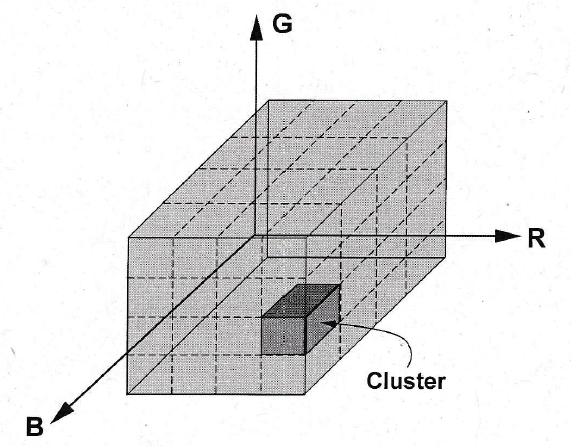
\includegraphics[scale=0.4]{3_66}
	\item Pre-clustering procedure:
	\begin{itemize}
		\item divides the color space into a certain amount of clusters
		\item the color of a cluster is one color of the color palette
		\item RGB color space is uniformly divided into 256 colors without considering whether the colors exist in the real image or not
		\item this method delivers unsatisfying outcomes
	\end{itemize}
	\item Popularity algorithm:
	\begin{itemize}
		\item one of the algorithms to create an adapted color palette
		\item a histogram of colors is created: it is examined how often every color exists in the original image \\
		$\rightarrow$ A new color palette is generated out of m(=number of the desired color depth, e.g. 256) mostly used colors \\
		$\rightarrow$ the colors of the new palette are associated with the original colors of the image i.e. the colors of the palette which fit best the original color \\
		$\rightarrow$ the rest of the image colors is replaced by the one from the palette, which is very close to it (to determine the most similar color, the Euclidian distance is calculated)
		\item drawback:\\
		very time consuming; no structure is created so the complete color palette has to be searched for every color assignment \\
		any color details in small segments of the image could be completely wrong
	\end{itemize}
	\item Median-cut algorithm:
	\begin{itemize}
		\item In order to find the colors for the adapted color palette, the best approximation of the available colors is created instead of choosing colors from the original image
		\item all colors from the original image are marked in the RGB color cube \\
		$\rightarrow$ the cube is reduced in size until the cloud of marked colors fits the cube best \\
		$\rightarrow$ the cube is cut parallel to its longest edge(median-cut) in such a way that every sub-cube contains the same number of pixels \\
		$\rightarrow$  both sub-cubes are contracted until they fit exactly the number of pixels \\
		$\rightarrow$ again, the sub-cubes are cut along the median line and procedure recurs \\
		The procedure stops when a previously defined number of cub-cubes is reached
		\item in the best case, the resulting segments of the RGB color cube contain only one color that can be assigned to the pixels
		\item if more than one color is in the final cube, a mean value is calculated
	\end{itemize}
\end{itemize}

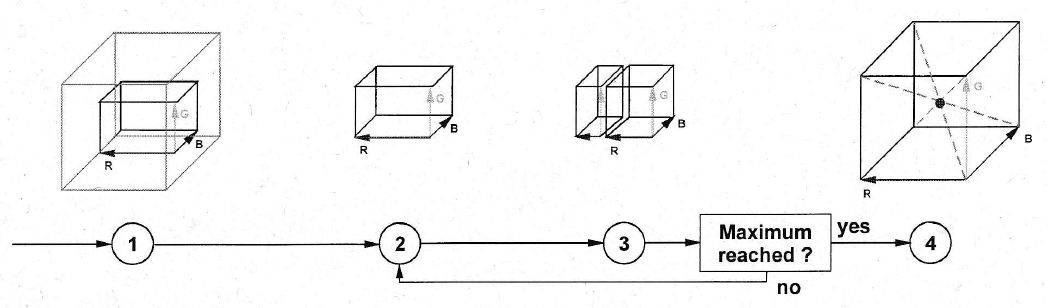
\includegraphics[scale=0.5]{3_69}

\begin{itemize}
	\item after the determination of the color palette, the difference(failure) between the needed(real) color and the associated color of the palette is not taken into account
	\item Floyd-Steinberg algorithm:
	\begin{itemize}
		\item in order to remove the remaining color steps, smoothens the color transitions
		\item the algorithm spreads this failure to the point of the neighborhood with the following weight: \\
		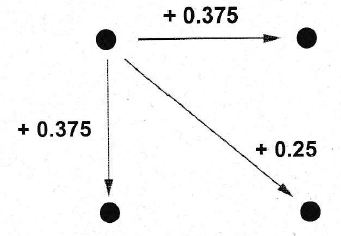
\includegraphics[scale=0.5]{3_71}
		\item the failures are gradually spread over the complete image without increasing the possible amount of palette colors
	\end{itemize}
\end{itemize}


\setcounter{subsection}{9}
\subsection{Calculation of Object's Visibility}

\begin{itemize}
	\item \textbf{visibility problem}: correct selection of polygons for a 3D scene, which are visible from a given view point
		\begin{itemize}
			\item only a small amount of polygons are visible.
			\item but viewpoint change rapidly $\rightarrow$ \textbf{real-time selection} is crucial
			\item algorithms for the object space vs. algorithms for the image space
				\begin{itemize}
					\item object space: work on the level of the objects with the same accuracy the objects have.
					\item image space: work on the level of the rasterized image with a resolution of one pixel
				\end{itemize}
		\end{itemize}
	\item \textbf{Culling procedure}: calculate the invisible lines and surfaces of the objects in a scene.
		\begin{itemize}
			\item view frustrum culling: all objects outside the viewing cone will be removed
			\item back face culling: the back faces of an object are removed
			\item occlusion culling: all objects that are hidden by an other one, are removed
		\end{itemize}
\end{itemize}

\subsubsection{View Frustrum Culling}

\begin{itemize}
	\item using a view cone: all objects inside frustrum have to be calculated. objects are on the border of the frustrum will only be partly calculated
\end{itemize}

\begin{figure}[H]
	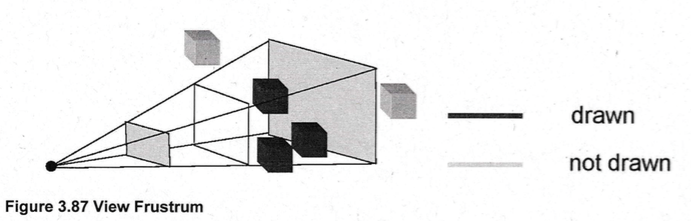
\includegraphics[width=\linewidth]{3_87}
\end{figure}


\subsubsection{Back Face Culling}

\begin{itemize}
	\item surfaces of an object facing away from the user will be removed
	\item z-component of the polygon's perpendicular has to be checked. (positive: faces away from the user - invisible)
\end{itemize}

\begin{figure}[H]
	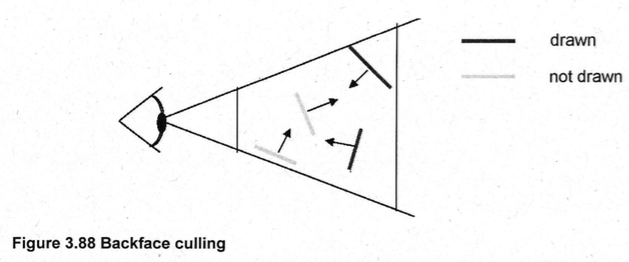
\includegraphics[width=\linewidth]{3_88}
\end{figure}


\subsubsection{Occlusion Culling}

\begin{itemize}
	\item all objects which are completely hidden by other objects from a given viewpoints are removed
	\item in principle, depth information is used for occlusion culling.
\end{itemize}

\subsubsection*{Priority Algorithms (painter algorithm)}

\begin{itemize}
	\item surfaces of an object are sorted concerning their depths, and displayed from the back to the front. (only elements on the top are visible)
	\item every surface has to be checked. 
\end{itemize}

\subsubsection*{Ray Tracing Algorithms (Ray Casting)}

\begin{itemize}
	\item rays from the center of projection into the scene are traced. (for every pixel in the image plane)
	\item intersection points of a ray with an object are calculated:
		\begin{itemize}
			\item tracing a ``light ray" in the backward direction from the center of projection to a pixel in the scene.
			\item determining the pixel's color by looking up the color of the hidden object in the scene.
			\item if a pixel does not have any intersection point, it will have the same color as the background.
			\item in all other cases, the intersection point is calculated, which is closest to the image plane.
		\end{itemize}
	\item +) for properties such as transparency and reflection, the color value of a pixel could be calculated. (raytracers)
\end{itemize}


\subsubsection*{z-Buffer Algorithm}

\begin{itemize}
	\item z-value (depth) of the displayed point is also stored:
		\begin{enumerate}
			\item all value of the depth buffer is set to $(-) \infty$
			\item for each surface of a polygon, depth info. of every point in the plane is calculated. At first, calculate for the corner points then arbitrary point in the middle of a polygon defined as follows:
			
			\begin{equation}
				z = \frac{-D - Ax - By}{C}
			\end{equation}
			
			\item if the depth of a calculated pixel is smaller than the value that is already stored, update to the newly calculated value.
			\item iterate 2, 3 for every polygons
		\end{enumerate}
	\item benefits:
		\begin{itemize}
			\item the order of the sampled polygons is arbitrary.
			\item the algorithm is independent of the complexity of the individual objects. 
			\item it is possible to add objects into scenes that are already rendered.
			\item the slow algorithm can be accelerated by implementing it into hardware
		\end{itemize}
	\item drawbacks:
		\begin{itemize}
			\item a large amount of memory is needed $\rightarrow$ solution: can be reduced by dividing the image into multiple rectangles and separately calculating. (parallel)
			\item exact smoothing, reflection and transparency are not possible. (object per pixel can be stored) $\rightarrow$ solution: every pixel is divided into n x n sub-pixels and edge is calculated on the level of the sub-pixels. An average color is calculated from the sub-pixels. 
			\item limited resolution. Object with a large extension in depth, sometimes the same value of z appears.
		\end{itemize}
\end{itemize}

\begin{figure}[h]
	\centering
	\begin{subfigure}[b]{0.45\textwidth}
		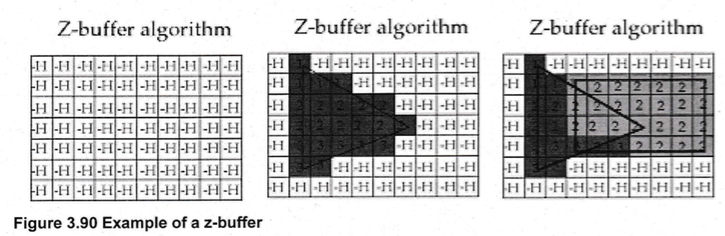
\includegraphics[width=\linewidth]{3_90}
	\end{subfigure}
	\begin{subfigure}[b]{0.45\textwidth}
		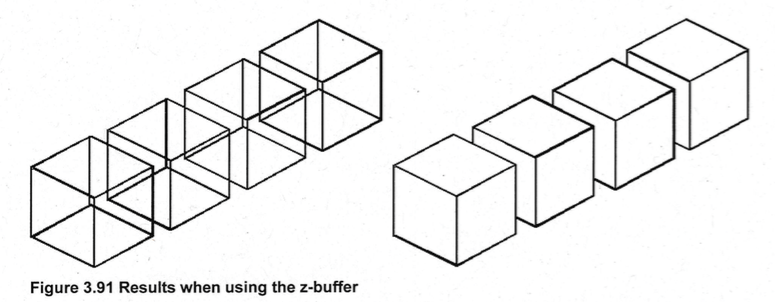
\includegraphics[width=\linewidth]{3_91}
	\end{subfigure}
\end{figure}

\subsection{The Distance Dependent Resolution (Level of Detail)}

\begin{itemize}
	\item the object far from the user $\rightarrow$ no need to simulate details
	\item the object covering the complete field of view $\rightarrow$ has to be displayed with more details
\end{itemize}

\begin{figure}[H]
	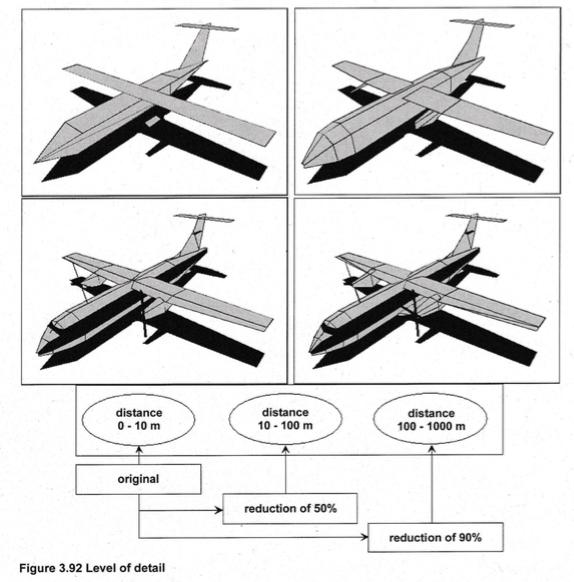
\includegraphics[width=\linewidth]{3_92}
\end{figure}


\subsection{Illumination Models}

\begin{itemize}
	\item photo-realistic quality $\rightarrow$ illumination model
	\item physical properties of light (Figure 3.93)
		\begin{itemize}
			\item diffuse reflection: uniformly scattered into all directions. The intensity depends on the perpendicular of the surface and on the direction of the incoming light.
			\item complete reflection: angle of incoming light = angle of reflected light. (color and the size of the reflection spot depends on the material)
			\item transmission: coupled with refraction. Global illumination models capture transmission.
		\end{itemize}
	\item rendering of light and shadow is affects by			
		\begin{itemize}
			\item light source type
			\item geometry, position of light source and camera
			\item geometry of the light, curvature of the geometry
			\item surface properties of the illuminated scenery (e.g. transparency, color, reflections)
			\item medium that transports the light (e.g. air, fog)
		\end{itemize}
\end{itemize}

\begin{figure}[H]
	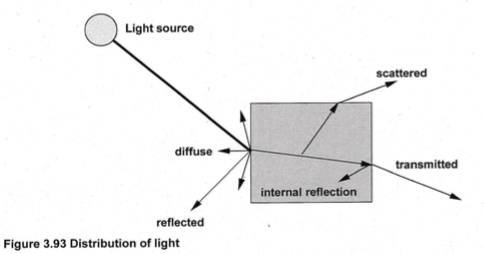
\includegraphics[width=\linewidth]{3_93}
\end{figure}

\subsubsection*{Light sources}

Figure 3.95

\begin{itemize}
	\item ambient light: background illumination. No defined light source and has no direction
	\item distant light: parallel light into one direction. The intensity of the light does not decrease with the distance from the light source
	\item spatial light: parallel light but decreases with the distance. (make smooth shadows)
	\item point light: light into every direction. The intensity decreases with the distance from the light source. (e.g. a simple bulbs)
	\item spotlight: cone-shaped light. The direction, position and dimension of the cone have to be defined.
\end{itemize}

\subsubsection*{Local vs. Global}

\begin{itemize}
	\item two different approaches for calculating the lighting of a scenary. 
	\item local: behavior of one point of the surface depending on the incoming light
	\item global: whole scenery together with the distribution of light
\end{itemize}

\subsubsection{Local Illumination Models}

\begin{itemize}
	\item calculates light intensity of a point on the surface of an object independently. 
	\item fast but many compromises
	\item can be implemented by hardware
	\item light transport:
		\begin{itemize}
			\item ambient light. no direction, uniformly distributed. 
			\item light which reaches the surface of an object and uniformly reflected (in all directions)
			\item light with a defined direction. 
		\end{itemize}
	\item Note: See the figures in the lecture note.
\end{itemize}

\subsubsection*{Reflection with Ambient Light}

\begin{itemize}
	\item light doesn't have orientation and reflected uniformly from every surface
	\item not sufficient for the visualization of object.
	\item intensity:
		\begin{equation}
			I = I_a \cdot k_a
		\end{equation}
		
		where $I_a$ is the intensity of the ambient light and $k_a$ is the ambient reflection factor ($0 < k_a < 1$)
\end{itemize}

\subsubsection*{Diffuse Surfaces}

\begin{itemize}
	\item by point light which emits light into all directions
	\item reflection is regardless of the viewer's position
	\item Lambert's reflection law:
		
		\begin{align}
			I &= I_p \cdot k_d \cos{\theta} \\
			&= 	I_p \cdot k_d (\vec{N} \bold{\cdot} \vec{L})
		\end{align}
		
		where $\vec{N}$ is the normal vector of surface, the $\vec{L}$ points into the direction of the light source, $I_p$ is the intensity of the incoming light and $k_d$ is the diffuse reflection coefficient. ($0 < k_d < 1$)
	\item pale surfaces can be visualized very realistically. However the surface properties of many objects are not suitable.
\end{itemize}

\subsubsection*{Specular Surfaces}

\begin{itemize}
	\item varnished or polished surfaces. (light center reflection - highlights)
	\item depends on the geometry and the viewpoint of the user. (position of the user is important!)
	
	\begin{equation}
		I = I_p \cdot k_s \cos^n{\alpha}
	\end{equation}
\end{itemize}

\subsubsection*{Ambient + Diffuse + Specular}

\begin{itemize}
	\item sum all terms..
	\begin{align}
		I &= \text{ambient} + \text{diffuse} + \text{specular} \\ 
		&= I_a \cdot k_a + I_p \cdot k_d \cos{\theta} + I_p \cdot k_s \cos^n \alpha \\
		&= I_a \cdot k_a + f_{att} \cdot I_p \big(k_d \cdot \cos \theta + k_s \cdot \cos^n \alpha \big) \\
		&= I_a \cdot k_a + f_{att} \cdot I_p \big(k_d \cdot (\vec{N} \bold{\cdot} \vec{L}) + k_s \cdot (\vec{R} \cdot \vec{V})^n \big)
	\end{align}
	
	where the factor $k$ and the exponent $n$ (shininess) depend on the kind of surface and influence the shape of the highlight.
	\item $\cos ^n \alpha$ heuristically approaches the scattering of the reflected light.
	\item attenuation element $f_{att}$: represents the decrease of the light intensity with an increasing distance to the light source ($d_L$): 
	
	\begin{equation}
		f_{att} = \frac{1}{d_L^2}
	\end{equation}
	
	\item refer to Figure 3.101
	\item note that the model is based on simplified assumptions for the physical properties of the surface. (other factors: microstructure of the surface, transparency of the material, wavelength of light...)
\end{itemize}

\begin{figure}[H]
	\includegraphics[width=\linewidth]{3_102}
\end{figure}


\subsubsection*{Approximation and Shading methods}

\begin{itemize}
	\item calculating illumination model only for the edges of the triangle, and all points in between are only interpolated. $\rightarrow$ saving time, good approximation to the local illumination model.
	\item flat shading (constant shading): if no apprx. is made between the corners of the triangle.
	\item alternatives: two methods for interpolation - Gouraud and the Phong interpolation 
\end{itemize}

\subsubsection*{Flat Shading}

\begin{itemize}
	\item Figure 3.106
	\item no apprx.
	\item illumination model used for one point of the polygon and all points of the polygon are assigned to the calculated color. 
	\item works well when...
		\begin{itemize}
			\item the light source is infinitely far away ($\theta = \text{const.}$)
			\item the viewer is infinitely far away ($\alpha = \text{const.}$)
			\item polygon represents the true surface of the object and not an approximation of a curved surface (no curved surface)
		\end{itemize}
	\item very fast but not realistic especially for ball.
	\item Mach-effect: two neighboring polygons with different shadings also have different intensities along their common edges. (problem!)
		\begin{itemize}
			\item Figure 3.107
			\item reason why the curved surfaces are not realistic in flat shading
		\end{itemize}
\end{itemize}


\subsubsection*{Gouraud shading}

\begin{itemize}
	\item color and intensity interpolation (apprx.)
	\item does not shade every polygon but treats it as part of a larger surface. (vertices)
	\begin{enumerate}
		\item vertex perpendicular is calculated for every vertex of the polygon grid.
			\begin{equation}
				N_V = \frac{\sum_{i=1}^n N_i}{\abs{n \sum_{i=1} N_i}}
			\end{equation}
		\item illumination model is applied to the vertices 
		\item intensity for the other points of the surface to be shaded by an interpolation of the other vertices.
			\begin{itemize}
				\item intensity for the points on the edges is calculated first by interpolating between the vertices. 
				\item inner area of the polygon can be shaded by interpolating between the intensities of the edges. (scan-line procedure: Figure 3.109)
				
				\begin{align}
					I_a &= I_1 - (I_1 - I_2) \frac{y_1 - y_s}{y_1 - y_2} \\
					I_b &= I_1 - (I_1 - I_3) \frac{y_1 - y_s}{y_1 - y_3} \\
					I_p &= I_b - (I_b - I_a) \frac{x_b - x_p}{x_b - x_a}
				\end{align}
				
			\end{itemize}
	\end{enumerate}
	\item drawbacks: shiny reflections could get lost due to the interpolation $\rightarrow$ Phong shading
\end{itemize}

\begin{figure}[H]
	\begin{subfigure}[b]{0.45\textwidth}
		\includegraphics[width=\linewidth]{3_109}
	\end{subfigure}
	\begin{subfigure}[b]{0.45\textwidth}
		\includegraphics[width=\linewidth]{3_112}
	\end{subfigure}
\end{figure}

\subsubsection*{Phong shading}

\begin{itemize}
	\item interpolation, but perpendiculars of the surfaces are interpolated instead of the intensities.
	\item very realistic but computationally expensive.
		\begin{enumerate}
			\item vertex perpendiculars of the polygon grid are calculated by using the mean value of the perpendiculars of the neighboring surfaces. 
			\item the perpendiculars is calculated by interpolation for every pixel of the surface to be shaded. (sperpendiculars of the pixels on the edges are interpolated from the vertex perpendiculars)
			\item perpendiculars of the inner polygon pixels are calcualted by a scan-line procedure.
			\item normalize and local illumination procedure is applied for every perpendicular. 
		\end{enumerate}
\end{itemize}

\subsubsection*{Interpolation methods}

\begin{itemize}
	\item Phong is time-consuming (more calculation)
	\item Phong is more realistic (more precise illumination)
	\item if the light hits the inner area without illuminating the corner, Gouraud does not work properly (all dark polygon)
	\item For both methods, the silhouette of the polygon is not very smooth. $\rightarrow$ subdividing the polygon into much smaller polygons. (but computation $\uparrow$)
	\item result of shading algorithms with interpolation depend on the orientation of the polygon. (Figure 3.114)
	\item if two neighboring polygons do not have any vertex on a common edge then it's problematic. (Figure 3.115)
	\item the geometry of the surfaces sometimes, is not represented very well by the vertex perpendiculars. In this case, light from very far distance will cause no change in shading. (Figure 3.116)
\end{itemize}


\subsubsection{Global Illumination Models}

\begin{itemize}
	\item consider the complete scenery: the relationship among objects is considered.
	\item very realistic(advantage) but dramatically higher computation time(drawback)
	\item transmission (incl. diffraction) and the exact distribution of diffuse light are global model
	\item cannot implemented in hardware (so many factors e.g. amount of light source, geometry complexity, medium...)
	\item two solution:
		\begin{itemize}
			\item Raytracing: calculate reflection, transparencies, refraction (w/o scattering) and shadows. Diffuse reflection is not supported well.
			\item Radiosity: only for diffuse reflection. (opague or diffuse radiator assumption)
		\end{itemize}
\end{itemize}

\subsubsection{Raytracing}

\begin{itemize}
	\item trace a light beam on its way from the source to the eye. (when calculating, eye to source since only a few light reach the eye)
	\item eye emits rays $\rightarrow$ if the ray strikes a surface it's reflected, changed in color, and partially absorbed. 
	\item uses optical laws for ideal reflection and refraction. 
	\item process stops under the conditions of:
		\begin{itemize}
			\item the ray strikes a light source
			\item the transported energy of the light ray is too low
			\item the ray leaves the scenery
		\end{itemize}
	\item shadow rays: towards the light source are calculated for the place, at which the initial ray hits upon the object. only if no solid object is between, the source illuminates the object directly.
	\item ray is emitted for every pixel until it strikes an object. $\rightarrow$ ray hits upon an object, the local illumination model is applied $\rightarrow$ two new rays are created: ideally reflected and the ideally refracted. $\rightarrow$ recursively calculate...
		\begin{enumerate}
			\item define the closest intersection point of the ray from the eye to any object
			\item calculate the ideally reflected ray
			\item calculate the light intensity of the reflected ray
			\item calculate the ideally refracted ray
			\item calculate the light intensity of the refracted ray
			\item calculate the shadow ray 
			\item interpretation of the illumination model in the examined location
		\end{enumerate}
	\item check Figure 3.120, 3.121, 3.122, 3.123
\end{itemize}

\begin{figure}[H]
	\centering
	\begin{subfigure}[b]{0.3\textwidth}
		\includegraphics[width=\linewidth]{3_120}
	\end{subfigure}
	\begin{subfigure}[b]{0.3\textwidth}
		\includegraphics[width=\linewidth]{3_121}
	\end{subfigure}
	\begin{subfigure}[b]{0.3\textwidth}
		\includegraphics[width=\linewidth]{3_122}
	\end{subfigure}
\end{figure}

\begin{figure}[H]
	\includegraphics[width=\linewidth]{3_123}
\end{figure}


\setcounter{subsubsection}{4}
\subsubsection{Radiosity}

\begin{itemize}
	\item how light (energy) is distributed in a virtual scenery?
	\item assumption: energy stays constant in a closed room 
		\begin{itemize}
			\item energy radiated from a surface = radiation (or radiosity)
			\item surface is assumed to be an opague, diffuse Lambert. 
		\end{itemize}
	\item radiosity equation: energy leaving is the sum of emiited and reflected light
		\begin{equation}
			B_i = E_i + \rho_i \sum_{i \leq j \leq n} B_j F_{j-1} \frac{A_j}{A_i}
		\end{equation}
		
		where:
		
		\begin{itemize}
			\item $B_i$, $B_j$ are the radiosities of the surface elements i and j, measured as energy per time unit and surface unit (W/m$^2$)
			\item $E_i$ is the emission rate. $> 0$ for light sources, else $0$
			\item $\rho_i$ is the reflection coefficient ($0 \leq \rho_i \leq 1$)
			\item $F_{j-1}$ is a form factor or configuration factor: the amount of energy, which leaves the element j and arrives at the element i. (shape, orientation and hindrance of both elements)
			\item $A_i$, $A_j$ are the areas of i and j
			\item $N$ is the amount of surface elements in a scenery.
		\end{itemize}
	\item approximation of the form factors: semi-cubes or hemispheres are used. (Figure 3.128)
	\item IMPORTANT read the page 3-108 to 3-115 carefully.
\end{itemize}

\subsection{Textures}

\begin{itemize}
	\item why texture? 
		\begin{itemize}
			\item creating realistic obj.
			\item creating surface properties
			\item visualize contours
			\item distinguish between different parts of an obj.
		\end{itemize}
	\item complex object (e.g. golf ball) needs large amount of polygons $\rightarrow$ texture is an efficient alternative
	\item how an image or a bitmap is applied to a polygon
	\item two methods to create texture
		\begin{itemize}
			\item designing texture manually
			\item mathematical methods
		\end{itemize}
\end{itemize}

\subsubsection{The Different Kinds of Textures}

\begin{itemize}
	\item classification 
		\begin{itemize}
			\item 2D vs 3D
		\end{itemize}
\end{itemize}

\subsubsection*{Bump Mapping}

\begin{itemize}
	\item within a bump map, the amount is stored by which the normals are changed towards the perpendiculars of the surfaces. (2D geometry is preserved, but normal vectors are changed)
	\item color, intensities are not changed
	\item bump map: array of shift values. 
	\item Bump-Mapping cannot be combined with interpolation illumination models: Phong, Raytracing (o) Gouraud (x) (After G., everything is changed into flat)
\end{itemize}

\subsubsection*{3D Texture}

\begin{itemize}
	\item AKA texture mapping: the textures on the surface of the object are a result of the several cuts in the 3D texture space.
\end{itemize}

\begin{figure}
	\includegraphics[width=\linewidth]{3_153}
\end{figure}


\subsubsection{The Mapping of Textures}

\begin{itemize}
	\item terms:
		\begin{itemize}
			\item texture plane: 2D plane in which the texture is defined
			\item object space: within 3D object space, the models are created that will be provided later with textures
			\item image field: contains the 2D completely rendered scenery
		\end{itemize}
\end{itemize}

\end{document}
%\documentclass{standalone}
% Load any packages needed for this document
\begin{document}
\section{Chapter 5 Hardware for VR}
complete VR installation consists of three main parts:
\begin{itemize}
\item User field: consists of various persons and/or application fields
\item Simulation field: consists of efficient computer(calculates presentation from the virtual environment) and also the feedback from the user
\item Interaction field:interaction field consists of the human-computer interface, which is used for the analog-in and output of the VR data 
\end{itemize}
\subsection{Visual In- and Output Devices}
\begin{itemize}
\item eye is the most important perception channel
\item Active Displays: generate the light for illumination(CRT, LED, VFD, plasma display)
\item use ambient light or background illumination(LCD)
\end{itemize}
\subsubsection{Display Technologies}
\subsubsection*{Cathod Ray Tube(CRT)}
\begin{itemize}
\item Developed by Ferdinand Braun at 1909
\item For multiple colors, penetron tube and mask tube is used
\begin{itemize}
\item Penetron Tube: works in the same way as cathod ray tube but different floresence colors are stacked at thte inside of the tube. In order to activate different layers, the electrons must have different kinetic energies.
\item Mask Tube: florescence colors are arranged in small triples or stripes(dots are visible if enlarged)
\end{itemize}
\item hole-mask or a slot-mask is used infront of the phosphoric layer which eliminates all unfocused electrons due to its positive charge
\item limitation of resolution is not given by cathod ray-tube but by the image is digitally processed
\begin{itemize}
\item vector technology: pros(no discretization, small amount of memory transformation in hardware) cons(only polygons, no surfaces, only low complexity otherwise image flicker)
\item grid technology: pros(surfaces can be displayed, simple and cheap, complex geometry possible) cons(visible steps, framebuffer needed, scan conversion needed) : ongoing technical development completely replaced by grid technology.
\end{itemize}
\end{itemize}
\subsubsection*{LC Displays}
\begin{itemize}
\item LC: Liquid Crystal in fluid state behaves like a fluid but also show some crystalline properties at the same time.
\item Three different states: nematic smectic, cholesteric
\begin{itemize}
\item Nematic: in nematic state all 
\end{itemize}
\end{itemize}
\subsubsection*{Ferroelectric Liquid Crystal Displays(FLCD)}
\subsubsection*{LED-Screens}
\subsubsection*{Plasma Displays(PDP)}
\subsubsection*{OLED Techonology}
\subsubsection*{Field Emission Display}
\subsubsection*{Electronic Paper}
\subsubsection*{Comparison between the Different Technologies}

\subsubsection{Projectors}
\subsubsection{Stereo Display Technologies}









\subsection{•}
\end{document}

\end{document}
